% =============================================================================
% FILE: fvpreport.tex
% =============================================================================

%
% Air University Kamra BS FYP Template
% Prepared By: Mustajab Hussain <mustajab@aack.au.edu.pk>
%
% Version History
% 0.1 11-07-2024
% 0.2 19-03-2025

\documentclass{air-kamra-bs}

\usepackage{blindtext}
\usepackage{mathptmx}% Times Roman font
\usepackage[T1]{fontenc}
\usepackage{lipsum} 
\usepackage{sectsty}
\usepackage{tikz-uml}
\usepackage{titlesec}
\usepackage{colortbl}
\usepackage{longtable}
\usepackage{tabularx}
\usepackage{array}
\usepackage{amssymb}
\usepackage{float}

\renewcommand{\arraystretch}{1.5}
\setlength{\tabcolsep}{5pt}

% Information about the fyp report
% CHANGE BELOW INFORMATION ONLY. 
% Do not change air-kamra-bs.cls file
% -----------------------------------------------------------------------------
%%%%%%%%%%%%%%%%%%%%%%%%%%%%%%%%%%%%%%%%%%%%%%%%%%%%%%%%%%%%%%%%%%%%%%%%%%%%%%%
\department{Department of Computer Science}
\university{Air University Aerospace \& Aviation Campus}
\faculty{Computer Science}
\degreeyear{2026}
\degreemonth{June}
\degreename{Computer Science}
\campuscity{Kamra}
\authorone{Muhammad Saad Zafar}{225161}{225161@aack.au.edu.pk}
\authortwo{Muhammad Hamayun Farasat}{225158}{225158@aack.au.edu.pk}
\authorthree{Hamza Tariq}{225184}{225184@aack.au.edu.pk}
\authoronefather{Zafar Iqbal}
\supervisor{Mr. Ghulam Ali}
\sessionduration{2022-2026}
\hodname{Dr. Head of Computer Science Department}
\fypcoordinatorname{Name of FYP Coordinator}
\title{NewsPulse: A News Aggregation and Analysis Platform}
%%%%%%%%%%%%%%%%%%%%%%%%%%%%%%%%%%%%%%%%%%%%%%%%%%%%%%%%%%%%%%%%%%%%%%%%%%%%%%%

%%%%%%%%%%%%%%%%%%%%%%%%%%%%%%%%%%%%%%%%%%%%%%%%%%%%%%%%%%%%%%%%%%%%%%%%%%%%%%
% Document starts below
\begin{document}

\begin{dedication}
    \begin{center}
        \textit{This engineering work is dedicated primarily to Almighty Allah, the source of all knowledge, wisdom, and strength.}\\ \vspace{0.5cm}
        \textit{It is further dedicated to our respected parents and family members, whose continuous sacrifices, unconditional support, and encouragement provided the stable foundation required to complete this software engineering endeavor. Finally, we dedicate this work to our friends and teachers who offered guidance, motivation, and support throughout our academic journey.}
    \end{center}
\end{dedication}

\begin{acknowledgements}
    The development and realization of the NewsPulse platform were made possible through the support, advice, and contributions of several individuals. 

    The authors express their deepest gratitude to their project supervisor, Mr. Ghulam Ali, for his excellent technical mentorship, analytical insights, and structured guidance. His deep understanding of distributed microservices architecture and natural language processing pipelines helped navigate numerous container scheduling and hardware optimization bottlenecks encountered during system deployment.

    Sincere appreciation is extended to our parents and families for their continuous moral support and patience, which allowed us to maintain the focus necessary to complete this project. We also thank our peers in the Department of Computer Science at Air University, Aerospace \& Aviation Campus Kamra, for fostering a highly collaborative and academically stimulating environment.

    Finally, the authors acknowledge the maintainers and contributors of the open-source software ecosystem—specifically FastAPI, PyTorch, React, and HuggingFace—whose foundational frameworks, tools, and libraries made the implementation of this secure, localized intelligence system possible.
\end{acknowledgements}

\begin{executiveSummary}
    The digital news ecosystem faces critical challenges from the rapid spread of misinformation and narrative bias. Traditional media intelligence platforms rely heavily on cloud-dependent, proprietary Large Language Models (LLMs), which introduce prohibitive operational costs, runtime latency, and data privacy vulnerabilities. This project introduces NewsPulse, a secure, self-hosted news aggregation and forensic analysis platform designed to execute entirely on resource-constrained consumer hardware. Deployed as a highly decoupled, 11-container microservices architecture orchestrated via Docker Compose, the platform delivers high-availability news indexing and deep text analytics locally, eliminating external API dependencies.

    At the core of the platform is a resilient, asynchronous data ingestion pipeline that aggregates raw articles from global feeds using a background daemon powered by APScheduler. Payloads are extracted through a three-stage fail-safe parser (spoofed async HTTPX requests $\rightarrow$ native Trafilatura HTML parsing $\rightarrow$ direct raw \texttt{urllib3} socket connections with disabled TLS verification). Aggregated articles undergo multi-signal analytical evaluations: fake news detection is computed via a Sentinel consensus heuristic that weights fine-tuned deep learning (BERT) classifiers, capitalization stylometrics, and Sensational Lexicon densities; political bias is tracked using a 512-token sliding window with 448-token overlap, weighting introductory/concluding tokens at 1.5x and applying an apolitical Topic Gate to filter objective categories.

    To guarantee high-throughput stability, the system incorporates strict operational boundaries, including 2,500-character input truncations and automatic fallbacks to a high-speed TF-IDF extractive summarizer during Out-of-Memory (OOM) alerts. Hallucination-free counter-arguments are generated by a Socratic Debater engine integrating an INT8 quantized Flan-T5 model with dynamic post-inference lexical filters and regex-based proper-noun template backups. Finally, data privacy is enforced using end-to-end payload cryptography, which encapsulates transient AES-256-GCM symmetric session keys via public RSA-2048 keys (RSA-OAEP with SHA-256) between the React client and FastAPI Uvicorn gateway, securing sensitive analyst workflows.
\end{executiveSummary}

\begin{abstract}
    Automated media aggregation and analytical platforms are crucial for counteracting misinformation and identifying narrative bias. However, existing solutions rely heavily on cloud-connected models that introduce significant data sovereignty risks, high recurring operational costs, and latency overheads. This project details the design and deployment of NewsPulse, a decentralized, 11-container microservices platform orchestrated via Docker Compose. The architecture routes all client communication through a high-performance FastAPI gateway. The gateway decrypts incoming payloads and coordinates stateless downstream analysis across CPU-bound Natural Language Processing (NLP) inference containers.

    Core functionalities include asynchronous article ingestion from external feeds with fallback scrapers, multi-signal fake news consensus detection, topic-gated political bias evaluation, and template-driven Socratic debater engines. Operational stability is enforced through strict character-level input boundary truncations and deterministic Term Frequency-Inverse Document Frequency (TF-IDF) fallbacks to prevent container Out of Memory (OOM) failures under heavy multi-user workloads. Cryptographic security is achieved by deploying hybrid end-to-end payload encryption using AES-256-GCM symmetric session keys and RSA-OAEP asymmetric key encapsulation. Quality assurance was validated through pytest frameworks, regression suites, and stress tests under concurrent user loads. Multi-process Gunicorn metrics are continuously aggregated via Prometheus and rendered on Grafana dashboard panels. The resulting system delivers low-latency, hallucination-free news intelligence, establishing a secure and highly scalable deployment model for constrained hardware.
\end{abstract}

\chapter{Introduction \& Background}
\label{sec:introduction-background}
\newpage

The contemporary digital landscape has fundamentally transformed how information is distributed and consumed. The transition from traditional print and scheduled broadcast media to real-time digital syndication has compressed the news lifecycle, enabling instantaneous updates but simultaneously accelerating the propagation of unverified claims, polarized narratives, and coordinated misinformation. processing this massive volume of high-velocity textual data in real-time presents a severe challenge for standard media analysis systems. Manual fact-checking pipelines cannot scale to handle this throughput, while conventional automated solutions rely on massive, monolithic artificial intelligence models that introduce prohibitive operational costs and high inference latency.

This chapter introduces NewsPulse, a highly decoupled, microservices-based intelligence platform engineered to aggregate, summarize, and analyze news articles along multiple dimensions. Designed to operate within strictly constrained local hardware environments, NewsPulse circumvents the need for expensive, GPU-accelerated cloud architectures and proprietary generative model APIs. By utilizing highly optimized, CPU-friendly HuggingFace Transformers, PyTorch dynamic integer quantization, and robust deterministic natural language processing fallbacks, the system executes sub-second multi-dimensional analysis on consumer-grade central processing units. The platform coordinates these stateless analytic engines behind an API gateway secured with end-to-end payload encryption, exposing operational insights via local telemetry tools.

\section{Background}
Automated computational journalism has traditionally depended on centralized, monolithic architectures to collect, classify, and distribute digital news. These monolithic systems struggle with scalability when subjected to modern concurrent traffic loads, as a performance bottleneck in one pipeline component (such as model loading or tokenization) can degrade the entire application's availability. Furthermore, the modern news ecosystem is heavily saturated with sensationalist styling and politically polarized framing, which standard statistical text classifiers frequently misinterpret.

To address these vulnerabilities, modern software engineering favors the decomposition of complex platforms into isolated, stateless microservices. When combined with local machine learning models, this microservices paradigm allows specialized containers to scale independently based on their specific CPU or memory usage. To ensure the trustworthiness of the automated metrics, these models must provide explainable visual feedback (Explainable Artificial Intelligence or XAI) rather than returning opaque scalar indicators. In resource-constrained deployment environments lacking dedicated hardware accelerators (such as graphics processing units or tensor processing units), this microservice topology must be fortified with deterministic, low-overhead fallback heuristics to maintain continuous availability under heavy system load.

\section{Motivation and Challenges}
The core engineering challenge addressed by this project is the construction and deployment of a multi-service NLP pipeline within severe local hardware restrictions, specifically targeting consumer-grade CPUs with restricted random-access memory. 

The primary technical challenges include:
\begin{itemize}
    \item \textbf{Resource Exhaustion and Tensor Overflows:} Large-scale transformer models easily saturate system memory when processing long-form journalism. When tokenizing articles exceeding standard sequence boundaries, traditional encoder-decoder pipelines can suffer from tensor indexing errors and out-of-memory crashes. NewsPulse addresses this constraint by implementing character-level hard truncation limits (e.g., capping summarizer inputs at 2500 characters) and processing long texts through overlapping 512-token sliding window arrays to ensure safe and stable execution.
    \item \textbf{Data Heterogeneity and Network Blocking:} Digital news feeds frequently supply incomplete payloads or truncated description snippets. Furthermore, standard scraping tools often trigger security blocks, TLS handshake timeouts, and anti-bot defenses. To bypass these limitations, this project designs a resilient, multi-tiered crawler that sequentially falls back from an async HTTP client with randomized user-agent spoofing to a native scraping engine, and ultimately to an unverified TLS connection bypassing certificate checks.
    \item \textbf{Explainability Deficits in Black-Box Models:} Standard deep-learning classification models function as mathematical black boxes, outputting bias or credibility scores without explaining the specific linguistic triggers. This lack of transparency prevents users from critically evaluating the system's conclusions. The system resolves this challenge by computing localized, sentence-level stylometric sensationalism metrics and identifying highly biased token sequences to highlight specific triggering sentences for the end-user.
    \item \textbf{Payload Transit Vulnerability:} Transmitting sensitive user preferences, reading histories, and raw analytics requests in cleartext exposes the system to traffic interception and profiling. To protect user data privacy without introducing significant latency, the architecture integrates a robust hybrid cryptosystem that handles asymmetric and symmetric encryption directly between the client interface and the gateway service.
\end{itemize}

\section{Goals and Objectives}
The primary objective of the NewsPulse system is to build a highly optimized, local intelligence engine that delivers real-time news collection and multi-dimensional analysis. The functional objectives of the platform are defined as follows:

\begin{enumerate}
    \item \textbf{Asynchronous Multi-Source Aggregation:} Engineer a localized background daemon utilizing asynchronous event loops to poll news APIs and RSS feeds every 15 minutes. The engine must clean the scraped HTML, classify the articles into distinct categories using keyword heuristics, deduplicate the stories using fast string normalization, and cache the processed array in Redis to serve as a zero-latency landing feed.
    \item \textbf{Hardware-Optimized Summarization:} Implement an abstractive summarization service using a local DistilBART model. To prevent resource saturation, the service must enforce character-level input limits. If the deep-learning model fails or system memory is depleted, the service must seamlessly fall back to a deterministic extractive algorithm that scores sentences based on term frequency with a square-root sentence length penalty.
    \item \textbf{Multi-Signal Consensus Credibility Assessment:} Deploy a consensus architecture (the Sentinel engine) that determines credibility by combining five distinct signals: localized BERT classification, custom stylometric density analysis (sensational vocabulary, capitalization ratios, exclamation densities, and clickbait patterns), cognitive complexity metrics (lexical diversity and subjectivity ratios), domain credibility scales, and live fact-check verification queries.
    \item \textbf{Context-Aware Bias Detection:} Develop an analytical service to estimate political polarization using a DistilRoBERTa model trained on news bias datasets. The model must process articles via overlapping 512-token windows and compute a weighted average of chunk probabilities, emphasizing the introduction and conclusion segments. The service must integrate an apolitical topic gate to suppress false-positive bias scores on sports, technology, and science journalism.
    \item \textbf{Quantized Socratic Debater Engine:} Construct a counter-argument generator powered by a quantized sequence-to-sequence model (LaMini-Flan-T5) optimized via PyTorch Dynamic INT8 Quantization. The system must post-process the generated text to eliminate model loop repetitions and grammatical errors, and fall back to a deterministic rule-based template engine that extracts proper nouns and matches domains if resources are exhausted.
    \item \textbf{Secure Cryptographic Transit:} Enforce comprehensive payload security using a hybrid cryptosystem. All communications between the client interface and the API gateway must be protected by encrypting payloads using AES-256-GCM, with the symmetric keys securely exchanged using RSA-2048 (OAEP-SHA256) standards.
\end{enumerate}

\section{Literature Review/Existing Solutions}
Recent research in automated news processing favors massive generative models hosted in cloud environments. While these models are highly capable, they introduce significant network latency, require substantial operational budgets, and expose sensitive user data to third-party providers. 

 bias detection systems documented in contemporary literature often utilize rigid, global token-classification matrices. Because these matrices do not account for domain-specific context, they frequently misclassify objective technical terms or highly descriptive sports commentary as politically biased. Furthermore, standard fact-checking and fake news detection applications rely on single-model predictions. By ignoring secondary stylometric markers, lexical diversity, or publisher track records, these applications remain highly vulnerable to adversarial text alterations and model hallucinations.

\section{Gap Analysis}
A rigorous evaluation of current news aggregation and analysis applications highlights three critical technological gaps:
\begin{itemize}
    \item \textbf{Unified Multi-Signal Classification:} Existing platforms separate aggregation, summarization, credibility evaluation, and bias detection into independent applications. No localized platform combines these processes into a unified analytical suite capable of running on standard hardware.
    \item \textbf{Explainable AI in News Analysis:} Modern analytics tools typically output binary classifications or scalar confidence scores without identifying the underlying textual evidence. The absence of sentence-level highlighting prevents users from understanding *why* a particular piece of journalism was flagged as biased or sensationalist.
    \item \textbf{System Telemetry and decoupling:} Most open-source news tools are built as monolithic applications that lack integrated performance monitoring. This makes it difficult to track system bottlenecks or model latency under concurrent load.
\end{itemize}

NewsPulse addresses these deficiencies by establishing a modular microservice architecture that isolates each analytical engine, implements sentence-level XAI highlighting, and integrates real-time telemetry tracking.

\section{Proposed Solution}
The proposed system is structured as an 11-container Dockerized ecosystem designed to decouple data ingestion, cryptographic security, stateful storage, and machine learning inference. 

\begin{figure}[h]
\centering
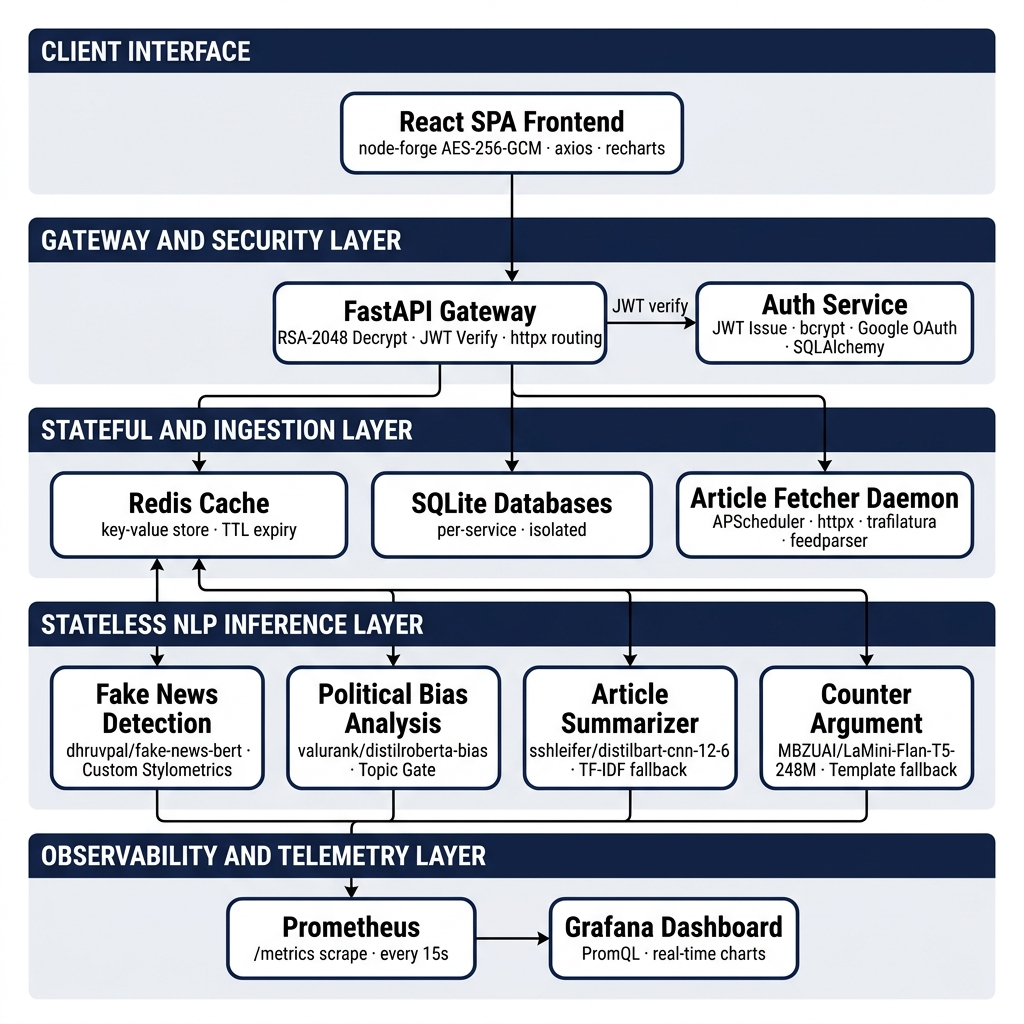
\includegraphics[width=\textwidth]{BS_FYP_Figs/system_architecture.png}
\caption{NewsPulse Decoupled Microservice Architecture}
\label{fig:sys_arch}
\end{figure}

The architecture is composed of the following core layers:
\begin{itemize}
    \item \textbf{Gateway and Authentication Layer:} Exposes a single entry point that validates JSON Web Tokens (JWT) and decrypts incoming asymmetric payloads. The service handles routing, payload unpacking, and error isolation.
    \item \textbf{Stateless Analytical Microservices:} Four independent containers host the Summarization, Fake News, Political Bias, and Counter-Argument services. Each container runs a highly optimized Python environment with specialized inference scripts, utilizing local directory paths for model weights to enable fast startup and offline operation.
    \item \textbf{Stateful Caching and Storage Layer:} Employs a local Redis instance as a high-speed broker to cache fetched articles, bias analyses, and summaries. Individual SQLite database instances are deployed inside each service container, ensuring that a database failure in one service does not affect the data persistence of the others.
    \item \textbf{Observability and Telemetry Stack:} Integrates Prometheus and Grafana. The system uses a specialized multi-process metrics collector to aggregate latency, request volumes, and cache hit ratios across all Uvicorn and Gunicorn worker threads.
\end{itemize}

\section{Project Plan}
The project implementation was structured using agile methodology, separating development into five sequential phases to ensure systematic integration and thorough verification of all sub-components.

\subsection{Work Breakdown Structure}
The system implementation tasks are divided into the following key phases:
\begin{itemize}
    \item \textbf{Phase 1 - Infrastructure and Cryptographic Setup:} Configuration of the Docker Compose multi-container environment, setup of the API Gateway, and implementation of the RSA-2048/AES-256-GCM hybrid encryption library.
    \item \textbf{Phase 2 - Asynchronous Ingestion Engine:} Development of the background article fetcher daemon, implementation of the multi-tier scraper fallbacks, and integration of the Redis cache.
    \item \textbf{Phase 3 - Analytical Model Optimization:} Integration of the local HuggingFace models, development of the TF-IDF and keyword-based fallback algorithms, implementation of PyTorch dynamic INT8 quantization, and configuration of the topic gates.
    \item \textbf{Phase 4 - User Interface Development:} Construction of the React frontend, integration of Recharts for bias and credibility visualization, and setup of the client-side cryptographic encryption routines.
    \item \textbf{Phase 5 - Telemetry Exposure and System Testing:} Configuration of Prometheus metrics export, creation of Grafana monitoring dashboards, and comprehensive performance testing under simulated user loads.
\end{itemize}

\subsection{Roles \& Responsibility Matrix}
The development tasks were distributed among the engineering team to support parallel progress across the frontend, gateway, and machine learning components.

\begin{table}[h]
\centering
\caption{Roles and Responsibility Matrix}
\label{tab:roles_matrix}
\renewcommand{\arraystretch}{1.2}
\begin{tabular}{|l|p{8.5cm}|}
\hline
\textbf{Team Member} & \textbf{Primary Responsibilities} \\ \hline
Muhammad Saad Zafar & NLP Inference Integration (Summarization, Fake News Detection, Counter Argument Generation), Local Model Optimization, API Gateway, Cryptographic Security \& Hybrid Encryption Layer \\ \hline
M. Hamayun Farasat & Background Ingestion Daemon (Article Fetcher Scraper), Political Bias Classification Model \& Sliding-Window Inference Pipeline \\ \hline
Hamza Tariq & React.js Frontend Interface Construction, Responsive Telemetry Dashboards, Recharts Visualization, and Frontend Client Cryptographic Integration \\ \hline
\end{tabular}
\end{table}

\subsection{Gantt Chart}
The developmental timeline spanned an eight-month lifecycle, coordinating parallel implementation tracks for the backend infrastructure, machine learning pipelines, and monitoring tools.

\begin{figure}[h]
    \centering
    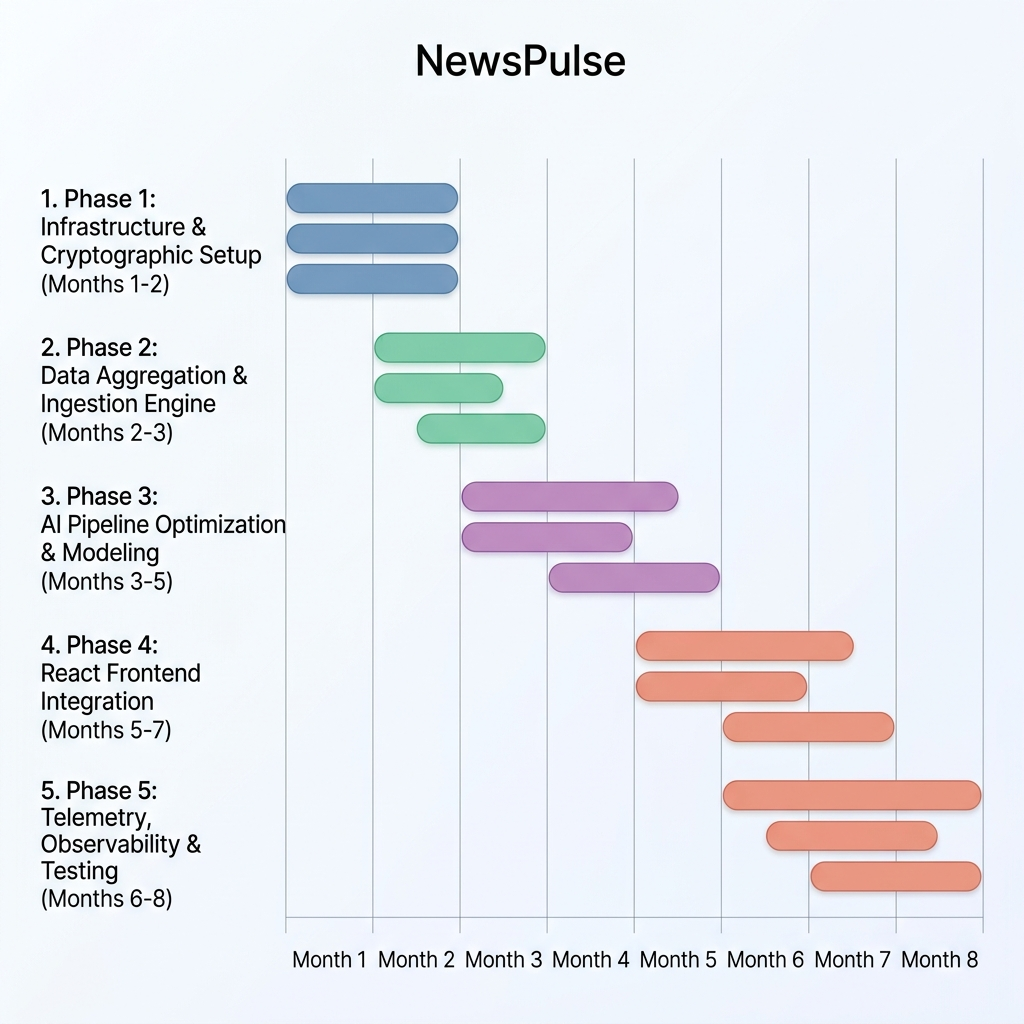
\includegraphics[width=\textwidth]{BS_FYP_Figs/gantt_chart.png}
    \caption{Project Implementation Gantt Chart}
    \label{fig:gantt_chart}
\end{figure}

\section{Report Outline}
The remainder of this document is structured into the following chapters:
Chapter 2 (Software Requirement Specifications) establishes the comprehensive functional and non-functional requirements of the system, detailing hardware/software boundaries, user characteristics, and structural constraints for localized deployment.
Chapter 3 (Use Case Analysis) provides a granular exploration of core system operations, presenting detailed actor behaviors, preconditions, execution flows, and exceptions for account actions and analytical pipelines.
Chapter 4 (System Design) documents the structural blueprints of the platform, including UML sequence diagrams, component configurations, centralized API gateway routing, and relational database schemas.
Chapter 5 (Implementation) details the core programming methodologies, explaining CPU-friendly transformer optimizations, PyTorch dynamic integer quantization, deterministic scraping heuristics, and hybrid cryptosystem integrations.
Chapter 6 (Business Plan) outlines the economic viability of the project, presenting target market demographics, monetization models, SWOT analysis, and operational cost projections.
Chapter 7 (Testing \& Evaluation) evaluates the platform's robustness under load, presenting functional validations, boundary testing outcomes, payload transit protection verifications, and real-time Prometheus telemetry.
Chapter 8 (Conclusion \& Future Work) summarizes the completed engineering milestones and technical contributions of the project, while presenting scalable paths for distributed crawling expansions.

\chapter{Software Requirement Specifications}
\label{ch:software-requirement-specifications}
\newpage

\section{Introduction}
This chapter defines the Software Requirement Specifications (SRS) for the NewsPulse platform. It establishes the functional and non-functional requirements that govern the architectural design, security boundaries, and local machine learning execution sequences within the decoupled microservices ecosystem.

\subsection{Purpose}
This document specifies the complete software requirements for the NewsPulse platform, a local news aggregation and multi-dimensional analysis engine designed to execute within strict hardware constraints without cloud-based Large Language Model (LLM) dependencies. The scope of these specifications encompasses the React client interface, the centralized FastAPI gateway, the high-speed Redis caching broker, and the suite of four stateless Natural Language Processing (NLP) inference containers. This document serves as the primary contract for development, quality assurance, system integration, and final project evaluation.

\subsection{Document Conventions}
The organization and structural formatting of this document conform to the IEEE 830-1998 standards for software requirements specifications. To maintain clarity across technical layers, specific typographical conventions are systematically applied:
\begin{itemize}
    \item \textbf{System Components and Directories:} Directory locations and software packages are denoted in a monospaced font (e.g., \texttt{/app/data}, \texttt{trafilatura}, \texttt{sqlalchemy}).
    \item \textbf{Cryptographic Protocols:} Asymmetric and symmetric security standards are capitalized in standard sans-serif notation (e.g., RSA-OAEP, AES-GCM).
    \item \textbf{Machine Learning Models:} Model identifiers and specific weights are formatted as literal strings (e.g., \texttt{sshleifer/\allowbreak{}distilbart-\allowbreak{}cnn-\allowbreak{}12-6}, \texttt{valurank/\allowbreak{}distilroberta-\allowbreak{}bias}).
    \item \textbf{Requirement Labeling:} Requirements are assigned unique identifiers (e.g., REQ-F01 for functional requirements, REQ-S01 for security requirements) to facilitate tracing and validation during system testing.
\end{itemize}

\subsection{Intended Audience and Reading Suggestions}
This document is prepared for software developers, backend engineers, system security auditors, database administrators, and the academic assessment panel. 
\begin{itemize}
    \item \textbf{Backend and AI Engineers:} Should focus on Section 2 (Functional Requirements), specifically the processing pipelines, token limits, and the deterministic fallback algorithms.
    \item \textbf{Security Auditors:} Should prioritize Section 3.1 (Security Requirements), examining the hybrid cryptographic key exchanges and payload encapsulation boundaries.
    \item \textbf{Frontend Developers:} Should review Section 3.2 (Usability Requirements) to understand the data-mapping schemas and the Explainable AI (XAI) text highlighting components.
    \item \textbf{Academic Evaluators:} Are suggested to read the Product Scope, followed by the Functional Requirements, and conclude with the Non-Functional Requirements to evaluate how the system handles severe resource constraints.
\end{itemize}

\subsection{Product Scope}
NewsPulse is designed to replace expensive, high-latency cloud-based generative AI systems with a suite of lightweight, CPU-optimized transformers and deterministic natural language processing fallbacks. The system automatically gathers news from public APIs and RSS feeds, caches the content, and runs parallel analytical pipelines. These pipelines evaluate fake news credibility, classify political bias using overlapping text windows, generate Socratic counter-arguments, and produce summaries. By performing all computations locally on standard central processing units (CPUs), the platform eliminates external API subscription costs. Communication security is maintained by encrypting all data transit between the client interface and the gateway using a hybrid asymmetric-symmetric cryptosystem.

\section{Functional Requirements}
The functional requirements specify the explicit operational capabilities that the NewsPulse microservices must execute.

\subsection{Ingestion and Cleaning Requirements}
\begin{itemize}
    \item \textbf{REQ-F01: Asynchronous Scheduled Aggregation} \\
    The system must operate an asynchronous aggregation daemon (\texttt{article\_fetcher}) running within a non-blocking background loop. Every 15 minutes, this loop must poll configured external sources (NewsAPI, NewsData.io, GNews, and RSS feeds) for new content. The daemon must parse the results, categorize each story into one of eight domains (General, Politics, Technology, Sports, Business, Entertainment, Health, Science) using keyword heuristics, deduplicate the stories using fast string normalization of URLs and titles, and write the active array to a Redis "hot\_news" key.
    \item \textbf{REQ-F02: Robust Multi-Tier Crawler Fallback} \\
    When fetching individual article bodies, the \texttt{article\_fetcher} must execute a three-tier connection degradation pipeline to bypass anti-bot locks, incomplete RSS feeds, and TLS restrictions:
    \begin{enumerate}
        \item \textit{Tier 1 (Primary):} An asynchronous HTTP client request utilizing randomized browser header spoofing.
        \item \textit{Tier 2 (Secondary):} A native scraping execution using the \texttt{trafilatura} download helper.
        \item \textit{Tier 3 (Tertiary):} A direct socket connection via a raw pool manager configured with unverified TLS settings (\texttt{cert\_reqs='CERT\_NONE'}) to bypass strict local handshake limitations.
    \end{enumerate}
    The system must discard scraped contents that fall below a minimum length of 100 characters.
\end{itemize}

\subsection{Analytical Processing Requirements}
\begin{itemize}
    \item \textbf{REQ-F03: Hardware-Safe Summarization with Heuristic Fallback} \\
    The summarization service must load a local instance of the \texttt{sshleifer/\allowbreak{}distilbart-\allowbreak{}cnn-\allowbreak{}12-6} model. To prevent out-of-memory errors on CPU instances, the input text must be truncated at the character level to a maximum of 2500 characters before tokenization. If the transformer pipeline fails or system memory is depleted, the service must execute a deterministic Term Frequency (TF) extractive algorithm. This fallback must tokenize sentences, filter out common English stop-words, score sentences based on token frequency normalized by the square root of the sentence length, and return the top five sentences.
    \item \textbf{REQ-F04: Multi-Signal Sentinel Credibility Consensus} \\
    The credibility engine must evaluate incoming texts using a multi-signal consensus formula rather than relying on a single classifier. The Sentinel engine must calculate a final fake news probability by combining:
    \begin{enumerate}
        \item \textit{Machine Learning Signal (45\%):} Probability score from a local BERT model (\texttt{dhruvpal/\allowbreak{}fake-\allowbreak{}news-\allowbreak{}bert}).
        \item \textit{Stylometric Signal (25\%):} Vocabulary sensationalism ratios, ALL-CAPS token densities, exclamation mark frequencies, and regex-based clickbait penalties.
        \item \textit{Cognitive Signal (20\%):} Lexical diversity and emotional vs. objective word ratios.
        \item \textit{Baseline Signal (10\%):} A neutral anchor value of 0.5.
    \end{enumerate}
    This raw consensus probability must be adjusted using a domain credibility multiplier (0.8x for trusted domains, 1.3x for low-trust sources). If the article title matches verified facts via live API searches, the probability must be scaled down to 25\% of the BERT score. If style is highly objective (style score < 0.1 and cognitive score < 0.3), the fake news probability must be capped at 0.49 to suppress false positive ML classifications. The service must output the sentence with the highest sensational density as the Explainable AI (XAI) highlight phrase.
    \item \textbf{REQ-F05: Window-Averaged and Topic-Gated Bias Classification} \\
    The political bias service must process text using a local DistilRoBERTa model (\texttt{valurank/\allowbreak{}distilroberta-\allowbreak{}bias}). Long articles must be parsed in overlapping 512-token windows (stride of 448 tokens, overlap of 64 tokens). The system must compute a weighted average of chunk probabilities, assigning a 1.5x weight to the introduction and conclusion chunks. To prevent false positives in apolitical domains, the service must run a "Topic Gate" keyword heuristic. If an article contains sports, science, or technology vocabulary without sufficient political anchor words, a Topic Penalty (0.3 to 0.7) must override the label to "Center" with high calibrated confidence. The service must also compute a Left/Right keyword framing index to determine the ideological direction.
    \item \textbf{REQ-F06: Hybrid Socratic Debater Engine} \\
    The counter-argument service must generate critical perspectives using a quantized sequence-to-sequence model (\texttt{MBZUAI/\allowbreak{}LaMini-\allowbreak{}Flan-\allowbreak{}T5-\allowbreak{}248M}) optimized via PyTorch Dynamic INT8 Quantization for local CPU execution. The input prompt must be capped at 250 words. The service must post-process the generated text by splitting it on sentence boundaries and filtering out repetitive loops, run-on sentences, grammatical negation errors, and dangling prepositions. If this generative pipeline fails, the service must execute a deterministic fallback that uses regex to extract proper nouns and matches domains to select a pre-defined Socratic template response.
\end{itemize}

\subsection{Monitoring Requirements}
\begin{itemize}
    \item \textbf{REQ-F07: Asynchronous Telemetry Collection} \\
    All FastAPI services must collect and expose operational metrics at a standardized \texttt{/metrics} endpoint. The services must use the \texttt{prometheus\_client} library configured with a specialized multi-process directory environment. This setup allows the Prometheus scraper to aggregate request counts, latency histograms, database performance, and cache hit ratios across multiple Uvicorn and Gunicorn worker threads.
\end{itemize}

\section{Non-Functional Requirements}
The non-functional requirements establish the performance, security, and portability standards for the NewsPulse platform.

\subsection{Security Requirements}
\begin{itemize}
    \item \textbf{REQ-S01: End-to-End Cryptographic Payload transit} \\
    All data transit between the React client and the FastAPI gateway must be encrypted to prevent traffic interception. The system must implement a hybrid cryptosystem:
    \begin{enumerate}
        \item \textit{Symmetric Layer:} Plaintext requests are encrypted using a transient 32-byte AES key in Galois/Counter Mode (AES-256-GCM) with a unique 16-byte initialization vector (IV) and a 16-byte authentication tag.
        \item \textit{Asymmetric Layer:} The AES key is encrypted using the gateway's public RSA-2048 key with Optimal Asymmetric Encryption Padding (OAEP) utilizing the SHA-256 hash function.
    \end{enumerate}
    The final payload must be transmitted as a single, Base64-encoded bundle containing the encrypted AES key (first 256 bytes), the IV (next 16 bytes), the ciphertext, and the authentication tag (last 16 bytes).
    \item \textbf{REQ-S02: Gateway-Level Token Validation and Time-Drift Allowance} \\
    The gateway must validate JSON Web Tokens (JWT) for all stateful user operations. To prevent authentication failures when deploying the system across distributed cloud nodes or virtual machines, the gateway's JWT validation routine must implement a \texttt{clock\_skew\_in\_seconds} allowance of 10 seconds to handle system time-drift.
    \item \textbf{REQ-S03: Relational Database Isolation} \\
    To prevent security breaches from escalating, each service must isolate its database credentials. SQLite databases must run inside separate container volumes, and passwords must be salted and hashed using the \texttt{passlib} library's \texttt{bcrypt} implementation before storage.
\end{itemize}

\subsection{Usability Requirements}
\begin{itemize}
    \item \textbf{REQ-U01: Dynamic Analytical Visualizations} \\
    The React user interface must display bias distributions, credibility scores, and category metrics using dynamic charts from the \texttt{recharts} library.
    \item \textbf{REQ-U02: Sentence-Level Explainable AI Highlight Rendering} \\
    The user interface must render the sentence highlighted by the credibility and bias engines as sensational or polarized. This text must be highlighted in the main article body to provide the user with clear visual evidence.
\end{itemize}

\subsection{Reliability Requirements}
\begin{itemize}
    \item \textbf{REQ-R01: Dual-Layer In-Memory and Redis Caching} \\
    Before running a forward pass on any local machine learning model, each service must check a local \texttt{TTLCache} and the shared Redis cache using a SHA-256 hash of the article text. If a cached analysis is found, the service must return it instantly to eliminate redundant CPU computation.
    \item \textbf{REQ-R02: Database Crash Isolation} \\
    The platform's microservices must interact with separate SQLite database files. A database crash, lock, or file corruption in one microservice (such as the political bias logging table) must not affect the operation of the other services.
\end{itemize}

\subsection{Maintainability/Supportability Requirements}
\begin{itemize}
    \item \textbf{REQ-M01: Decoupled Container Orchestration} \\
    The system infrastructure must be organized as an 11-container Dockerized ecosystem using Docker Compose. The services must be isolated into a dedicated bridge network. Modifying or updating a specific service (such as updating the political bias model files or changing the Socratic debater templates) must only require rebuilding that specific container without interrupting global gateway traffic.
\end{itemize}

\subsection{Portability Requirements}
\begin{itemize}
    \item \textbf{REQ-P01: Hardware-Independent CPU Execution} \\
    All NLP models and heuristics must run strictly on standard central processing units (CPUs). The platform must not require proprietary hardware acceleration platforms (such as NVIDIA CUDA) or cloud-based GPU instances, ensuring compatibility with standard, off-the-shelf consumer computers.
\end{itemize}

\subsection{Efficiency Requirements}
\begin{itemize}
    \item \textbf{REQ-E01: Character-Level Truncation Limits} \\
    To prevent system memory exhaustion and ensure predictable processing speeds on standard CPUs, all analytical containers must enforce strict character-level input limits (e.g., capping summarizer inputs at 2500 characters, which represents approximately 500-600 words).
    \item \textbf{REQ-E02: Non-Blocking Event Loop Thread Delegation} \\
    To ensure the FastAPI event loops remain responsive, the CPU-bound parsing operations (such as \texttt{trafilatura} HTML extraction and regex search arrays) must be offloaded to a designated local \texttt{ThreadPoolExecutor}.
\end{itemize}

\subsection{Domain Requirements}
\begin{itemize}
    \item \textbf{REQ-D01: Deterministic and reproducible Analysis} \\
    The system must generate deterministic, reproducible outputs to satisfy academic and journalistic integrity standards. By replacing generative LLM APIs with optimized, local, quantized models and rule-based template fallbacks, the system prevents random model hallucinations. The analytical results and summaries must remain strictly anchored to the source text.
\end{itemize}

\chapter{Use Case Analysis}
\label{ch:use-case}
\newpage

This chapter presents the functional interactions between the external actors and the NewsPulse platform. The system boundary, actor roles, and use case relationships are modeled to illustrate how the microservices coordinate authentication, background news ingestion, multi-signal credibility evaluation, political bias detection, and counter-argument generation. Each use case is supported by a detailed specification table that defines preconditions, execution flows, and fallback behaviors.

\section{Use Case Model}
This section describes the system boundary and the three primary actors that interact with the NewsPulse platform.

As shown in Figure~\ref{fig:use_case_main}, the architecture coordinates interactions among three primary actors:
\begin{itemize}
    \item \textbf{News Service Provider (External API):} A secondary actor representing the external news aggregation layers (NewsAPI, NewsData.io, and GNews) and RSS feeds. This actor interacts strictly with the automated background collection routines of the system.
    \item \textbf{End User (Client):} The primary human actor who interacts with the React client interface. The user must authenticate to access the natural language processing endpoints. Once authorized, the user can trigger background news feeds, run analysis on articles or URLs, and save analyzed reports.
    \item \textbf{System Administrator (Admin):} The operations actor who monitors container health, evaluates request latency histograms, and reviews Redis and SQLite memory constraints via the Grafana and Prometheus dashboards.
\end{itemize}

\begin{figure}[h]
    \centering
    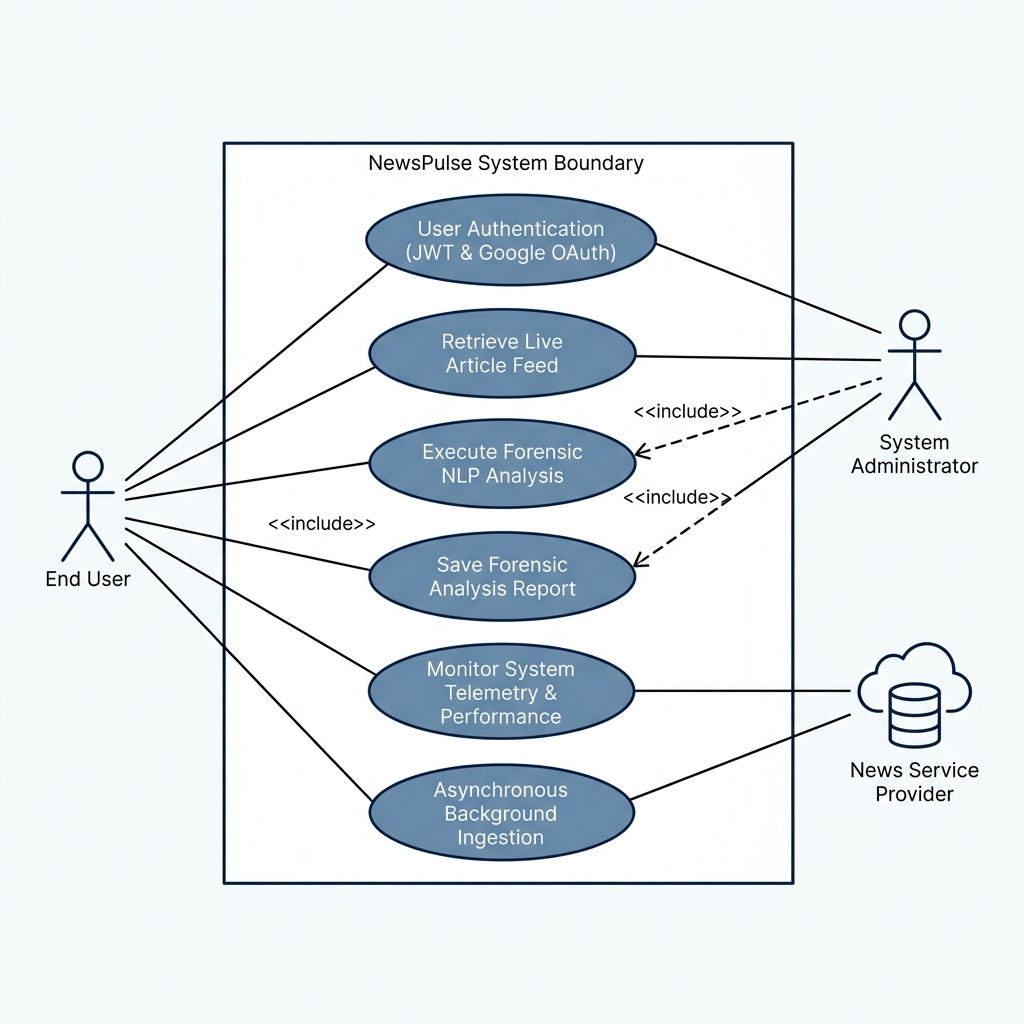
\includegraphics[width=0.85\linewidth]{BS_FYP_Figs/use_case_diagram.png}
    \caption{NewsPulse Decoupled System Use Case Diagram}
    \label{fig:use_case_main}
\end{figure}

The system boundary is governed by the centralized FastAPI Gateway. All stateful user interactions, such as running article analysis or saving reports, carry an \texttt{$\langle\langle$include$\rangle\rangle$} dependency on the validation of a valid JSON Web Token (JWT). Administrative telemetry operates in an isolated monitoring pipeline that does not expose secure user data.

\section{Use Cases Description}
This section describes the primary functional use cases of the NewsPulse microservices ecosystem. Each use case defines the actor, operational preconditions, the basic execution sequence, alternate flows for error and edge conditions, and the resulting post condition.

\subsection{User Registration and Authentication}
This use case manages user registration and authentication through the centralized \texttt{auth\_service}, verifying standard credentials or third-party Google OAuth tokens.

\begin{table}[h!]
    \begin{tabularx}{\textwidth}{|l|X|}
        \hline
        Title & Allow user to authenticate via standard credentials or third-party OAuth \\
        \hline
        Requirement & User must supply a valid username and password, or a verified Google identity token \\
        \hline
        Rational & To verify user identity and issue a signed JSON Web Token (JWT) for accessing the NLP microservices \\
        \hline
        Restriction or Risk & Time-drift on virtual machines hosting the containers may invalidate tokens prematurely \\
        \hline
        Dependency & SQLite authentication database, local Redis cache, active network interface \\
        \hline
        Priority & High (Critical Security Path) \\
        \hline
    \end{tabularx}
    \caption{User Authentication Function}
    \label{tab:table_user_login_function}
\end{table}

\subsubsection{Use Case 01: Standard Login}
This use case describes the step-by-step execution flow when a user authenticates using standard credentials or Google OAuth via the NewsPulse client.
\begin{table}[H]
    \renewcommand{\arraystretch}{1.3}
    \begin{tabularx}{\textwidth}{| X |}
        \hline
        \textbf{Standard Login and Authentication} \\
        \hline
        \textbf{Actor:}
        \begin{itemize}
            \item End User
            \item Google Identity Provider (for OAuth flow)
        \end{itemize} \\
        \hline
        \textbf{Preconditions:}
        \begin{itemize}
            \item The API Gateway and the \texttt{auth\_service} container are online and reachable.
            \item The local SQLite authentication database is connected via the SQLAlchemy engine.
        \end{itemize} \\
        \hline
        \textbf{Basic Flow:}
        \begin{itemize}
            \item The user submits credentials (username and password) via the client interface.
            \item The client encrypts the credentials using AES-256-GCM, wraps the symmetric key using the gateway's RSA-2048 public key, and transmits the Base64-encoded bundle.
            \item The API Gateway decrypts the payload using its private RSA key and forwards the credentials to the \texttt{auth\_service}.
            \item The \texttt{auth\_service} hashes the input password using \texttt{bcrypt} and compares it against the stored database hash.
            \item Upon successful validation, the gateway issues a JWT signed with HS256 and returns it to the client.
        \end{itemize} \\
        \hline
        \textbf{Alternate Flows:}
        \begin{itemize}
            \item \textbf{Alternate Flow 01 (Google OAuth):} If the user selects Google OAuth, the client sends a Google identity token. The gateway verifies it with Google's APIs, applying a 10-second clock skew allowance.
            \item \textbf{Alternate Flow 02 (Invalid Credentials):} If password validation fails, the gateway returns HTTP 401 Unauthorized and logs the failed attempt.
        \end{itemize} \\
        \hline
        \textbf{Post Condition:}
        \begin{itemize}
            \item The user receives a valid JWT token, enabling authorization for all subsequent NLP requests.
        \end{itemize} \\
        \hline
    \end{tabularx}
    \caption{Login Use Case}
    \label{tab:login_use_case}
\end{table}

\clearpage
\subsection{Execute Article Analysis}
This use case defines the execution sequence when an authorized user submits a raw article text block or URL for multi-signal analysis across the local NLP pipelines.

\begin{table}[h!]
    \begin{tabularx}{\textwidth}{|l|X|}
        \hline
        Title & Execute Multi-Signal Article Analysis \\
        \hline
        Requirement & User must present a valid, unexpired JWT \\
        \hline
        Rational & To generate article summaries, evaluate fake news credibility, map political polarization, and generate counter-arguments using local models \\
        \hline
        Restriction or Risk & Long-form text payloads may cause memory exhaustion and out-of-memory errors on standard CPUs \\
        \hline
        Dependency & Decoupled NLP microservices, Redis caching layer, isolated SQLite databases \\
        \hline
        Priority & High (Core Analysis Path) \\
        \hline
    \end{tabularx}
    \caption{Article Analysis Function}
    \label{tab:table_article_analysis_function}
\end{table}

\subsubsection{Use Case 02: Perform Article Inference}
This use case describes how the gateway coordinates the four parallel NLP containers to produce a complete forensic analysis of a submitted article.
\begin{table}[H]
    \renewcommand{\arraystretch}{1.3}
    \begin{tabularx}{\textwidth}{| X |}
        \hline
        \textbf{Multi-Signal NLP Article Inference} \\
        \hline
        \textbf{Actor:}
        \begin{itemize}
            \item Authenticated End User
        \end{itemize} \\
        \hline
        \textbf{Preconditions:}
        \begin{itemize}
            \item The user's JWT is verified by the gateway.
            \item The Summarizer, Fake News Detection, Political Bias, and Counter-Argument containers are online.
            \item The Redis cache container is active and reachable via the internal bridge network.
        \end{itemize} \\
        \hline
        \textbf{Basic Flow:}
        \begin{itemize}
            \item The user submits an article URL or text via the client interface.
            \item The client encrypts the request payload using AES-256-GCM and transmits it to the API Gateway.
            \item The gateway decrypts the payload, validates the JWT, and hashes the input text using SHA-256 to check the Redis cache.
            \item On a cache hit, the gateway returns the cached result immediately, bypassing the NLP models.
            \item On a cache miss, the gateway forwards the request in parallel to four NLP containers: Summarization (DistilBART-CNN-12-6), Fake News Detection (Sentinel BERT engine), Political Bias (DistilRoBERTa with windowed pooling), and Counter-Argument Engine (quantized Seq2Seq model).
            \item The gateway aggregates all outputs, writes the combined result to Redis, and returns the full analysis to the client.
        \end{itemize} \\
        \hline
        \textbf{Alternate Flows:}
        \begin{itemize}
            \item \textbf{Alternate Flow 01 (Input Truncation):} If the input text exceeds 2500 characters, the summarizer truncates the text to protect system memory.
            \item \textbf{Alternate Flow 02 (Heuristic Fallbacks):} If the DistilBART summarizer fails, a term-frequency sentence extraction algorithm is used. If the counter-argument engine fails, a template-based response is returned.
            \item \textbf{Alternate Flow 03 (Credibility Adjustments):} The credibility engine applies domain multipliers and caps objective styling scores at 0.49 to suppress false positive fake news classifications.
        \end{itemize} \\
        \hline
        \textbf{Post Condition:}
        \begin{itemize}
            \item The client receives the aggregated analysis, maps credibility and polarization using charts, and highlights the most sensational sentence using Explainable AI (XAI).
        \end{itemize} \\
        \hline
    \end{tabularx}
    \caption{Article Inference Use Case}
    \label{tab:article_inference_use_case}
\end{table}

\clearpage
\subsection{Manage Saved Articles}
This use case describes how an authenticated user persists a completed forensic analysis report to the local SQLite database for later retrieval.

\begin{table}[h!]
    \begin{tabularx}{\textwidth}{|l|X|}
        \hline
        Title & Save and Retrieve Forensic Analysis Report \\
        \hline
        Requirement & User must possess a validated, active JWT and a completed analysis \\
        \hline
        Rational & To allow users to store analyzed articles and access their history from the saved articles panel \\
        \hline
        Restriction or Risk & SQLite write locks under concurrent access may delay the save operation \\
        \hline
        Dependency & SQLite user database, SQLAlchemy ORM, active JWT session \\
        \hline
        Priority & Medium (User Persistence Path) \\
        \hline
    \end{tabularx}
    \caption{Manage Saved Articles Function}
    \label{tab:table_save_article_function}
\end{table}

\subsubsection{Use Case 03: Manage Saved Articles}
This use case describes the steps taken when a user saves a completed analysis report to their personal dashboard.
\begin{table}[H]
    \renewcommand{\arraystretch}{1.3}
    \begin{tabularx}{\textwidth}{| X |}
        \hline
        \textbf{Save Forensic Analysis Report} \\
        \hline
        \textbf{Actor:}
        \begin{itemize}
            \item Authenticated End User
        \end{itemize} \\
        \hline
        \textbf{Preconditions:}
        \begin{itemize}
            \item The user possesses a validated, active JWT.
            \item The forensic analysis for the target article has successfully completed.
        \end{itemize} \\
        \hline
        \textbf{Basic Flow:}
        \begin{itemize}
            \item The user selects the Save Article option on the client dashboard.
            \item The client encrypts the request and transmits it to the API Gateway.
            \item The gateway validates the JWT and forwards the payload to the user service.
            \item The user service connects to the SQLite database via SQLAlchemy and writes the analysis records to the saved articles table.
            \item The database confirms the write and the gateway returns HTTP 201 Created to the client.
        \end{itemize} \\
        \hline
        \textbf{Alternate Flows:}
        \begin{itemize}
            \item \textbf{Alternate Flow 01 (Database Lock):} If the SQLite database is locked by another thread, the SQLAlchemy engine retries with a 5-second timeout before returning HTTP 500.
        \end{itemize} \\
        \hline
        \textbf{Post Condition:}
        \begin{itemize}
            \item The analysis report is securely stored and the user can retrieve it later from the saved articles panel.
        \end{itemize} \\
        \hline
    \end{tabularx}
    \caption{Save Article Use Case}
    \label{tab:save_article_use_case}
\end{table}

\clearpage
\subsection{Monitor System Telemetry}
This use case describes how the System Administrator accesses real-time performance metrics via the Prometheus and Grafana monitoring stack.

\begin{table}[h!]
    \begin{tabularx}{\textwidth}{|l|X|}
        \hline
        Title & Access Container and System Telemetry \\
        \hline
        Requirement & Prometheus and Grafana containers must be active in the Docker bridge network \\
        \hline
        Rational & To give the administrator visibility into request latencies, CPU load, and Redis cache performance \\
        \hline
        Restriction or Risk & If a backend container goes offline, Prometheus marks its target as DOWN \\
        \hline
        Dependency & Prometheus, Grafana, backend \texttt{/metrics} endpoints, Docker bridge network \\
        \hline
        Priority & Medium (Operational Monitoring Path) \\
        \hline
    \end{tabularx}
    \caption{Monitor System Telemetry Function}
    \label{tab:table_telemetry_function}
\end{table}

\subsubsection{Use Case 04: Monitor Telemetry Metrics}
This use case describes the steps taken by the System Administrator to access and review real-time system performance data.
\begin{table}[H]
    \renewcommand{\arraystretch}{1.3}
    \begin{tabularx}{\textwidth}{| X |}
        \hline
        \textbf{Access Container and System Telemetry} \\
        \hline
        \textbf{Actor:}
        \begin{itemize}
            \item System Administrator
        \end{itemize} \\
        \hline
        \textbf{Preconditions:}
        \begin{itemize}
            \item The Prometheus and Grafana containers are active in the Docker bridge network.
            \item All backend containers are exposing their \texttt{/metrics} endpoints.
        \end{itemize} \\
        \hline
        \textbf{Basic Flow:}
        \begin{itemize}
            \item The Administrator opens the Grafana monitoring dashboard via the configured local port.
            \item Grafana queries the Prometheus time-series database for aggregated system metrics.
            \item Prometheus scrapes the \texttt{/metrics} endpoints of all backend services and aggregates Gunicorn and Uvicorn worker statistics via the \texttt{MultiProcessCollector}.
            \item The Administrator reviews system health metrics including request latencies, CPU utilization, and Redis cache hit ratios.
        \end{itemize} \\
        \hline
        \textbf{Alternate Flows:}
        \begin{itemize}
            \item \textbf{Alternate Flow 01 (Service Unreachable):} If a service is offline, Prometheus marks its target status as DOWN and triggers an alert in the Grafana dashboard, notifying the Administrator to restart the container.
        \end{itemize} \\
        \hline
        \textbf{Post Condition:}
        \begin{itemize}
            \item The Administrator obtains real-time system performance insights to manage container capacity and service availability.
        \end{itemize} \\
        \hline
    \end{tabularx}
    \caption{Telemetry Monitoring Use Case}
    \label{tab:telemetry_use_case}
\end{table}

\chapter{System Design}
\label{ch:system-design-chapter}
\newpage

This chapter details the architectural and logical formulation of the NewsPulse platform. It translates the software requirement specifications (SRS) and functional bounds of the system into a concrete engineering design, utilizing a highly decoupled 11-container microservices topology. The subsequent sections explore the system's structural and behavioral mechanics using standard Unified Modeling Language (UML) modeling. This includes mapping the localized natural language processing (NLP) pipelines, hybrid asymmetric-symmetric cryptographic data flows, isolated database aggregation schemas, and fault-tolerant degradation mechanisms designed to operate under strict hardware resource constraints.

\section{Architecture Diagram}
The system architecture rejects traditional monolithic designs in favor of a distributed containerized network orchestrated via Docker Compose. The architecture routes all client interactions through a centralized FastAPI gateway, which proxies requests to isolated, stateless Natural Language Processing (NLP) microservices. This separation isolates the CPU-bound HuggingFace \texttt{transformers} ecosystem from standard authentication and aggregation network traffic.

\begin{figure}[h!]
    \centering
    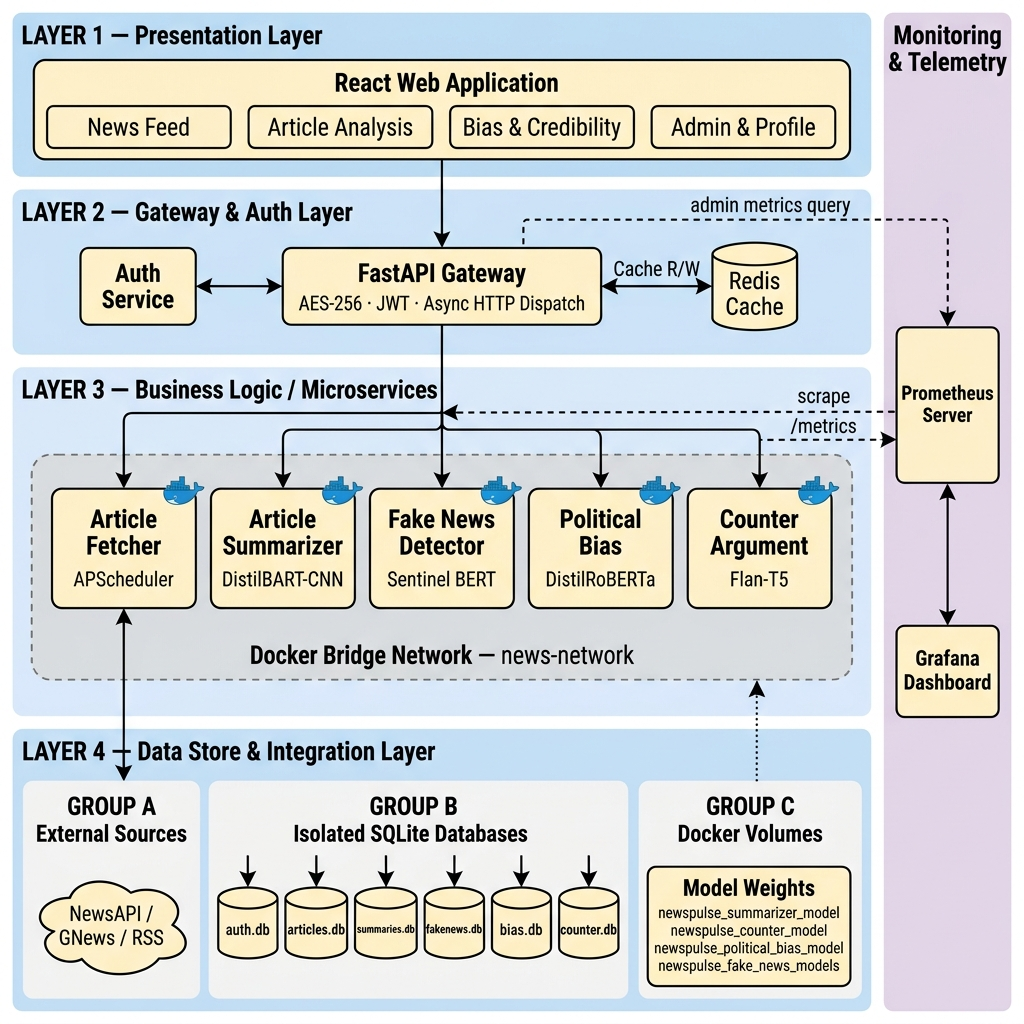
\includegraphics[width=1\linewidth]{BS_FYP_Figs/architecture_diagram.png}
    \caption{Architecture Diagram illustrating the 11-node microservices topology}
    \label{fig:architecture-diagram}
\end{figure}

As shown in Figure~\ref{fig:architecture-diagram}, the NewsPulse system is structured as an 11-node microservices topology divided into three primary tiers:
\begin{itemize}
    \item \textbf{Presentation Tier:} A single React-based single-page application (SPA) container running on port 3000 (mapped to port 80 inside Nginx). This tier renders the vector visualization dashboards and executes client-side cryptographic functions.
    \item \textbf{Gateway and Coordination Tier:} A central FastAPI Gateway container (port 8000) that serves as the single point of entry. It is allocated a resource boundary of 2.0 CPUs and 2 GB of RAM. The gateway decrypts incoming payloads using its private RSA-2048 key, performs user validation, checks JWT access tokens, and aggregates the multi-signal downstream results. It interfaces with an in-memory Redis caching container (port 6379, limited to 1.0 CPU and 2 GB of RAM) running `redis:7.4-alpine` to prevent duplicate inference passes.
    \item \textbf{Computational NLP Tier:} A suite of stateless FastAPI microservices operating within private Docker container environments:
    \begin{itemize}
        \item \texttt{article\_summarizer}: Bound to port 8001 (internal port 8000) with a limit of 4.0 CPUs and 8 GB of RAM. It generates summaries using a local instance of the \texttt{sshleifer/distilbart-cnn-12-6} model, storing weights in the persistent \texttt{newspulse\_summarizer\_model} volume.
        \item \texttt{fakenews\_detection}: Bound to port 8005 (internal port 8000) with a limit of 4.0 CPUs and 6 GB of RAM. It implements the Sentinel consensus algorithm, combining deep learning sequence classification from a local \texttt{dhruvpal/fake-news-bert} model with custom stylometric heuristics.
        \item \texttt{political\_bias}: Bound to port 8003 (internal port 8000) with a limit of 4.0 CPUs and 6 GB of RAM. It runs the \texttt{valurank/distilroberta-bias} model over overlapping sliding windows.
        \item \texttt{counter\_argument}: Bound to port 8002 (internal port 8000) with a limit of 2.0 CPUs and 4 GB of RAM. It generates critical perspectives using a PyTorch quantized \texttt{MBZUAI/LaMini-Flan-T5-248M} model, with \texttt{google/flan-t5-base} as a fallback.
    \end{itemize}
    \item \textbf{Ingestion Tier:} The \texttt{article\_fetcher} daemon container (port 8004) running with 1.0 CPU and 2 GB of RAM. It executes a background non-blocking aggregation loop every 15 minutes, scraping articles from public API feeds and RSS channels.
    \item \textbf{Telemetry Tier:} Comprises isolated Prometheus (port 9090) and Grafana (port 3001) containers. These services scrape operational metrics from the FastAPI \texttt{/metrics} endpoints to generate time-series dashboards.
\end{itemize}

\section{Domain Model Diagram}
The Domain Model establishes the vocabulary and logical boundaries of the computational journalism entities. The primary \texttt{Article} entity acts as the central node, correlating with specialized intelligence components including \texttt{Summarization}, \texttt{FakeNewsDetection}, \texttt{BiasedAnalysis}, and \texttt{CounterArgument}. These domain relationships map directly to the respective NLP pipelines rather than a centralized database, maintaining the principles of domain-driven design.

\begin{figure}[h!]
    \centering
    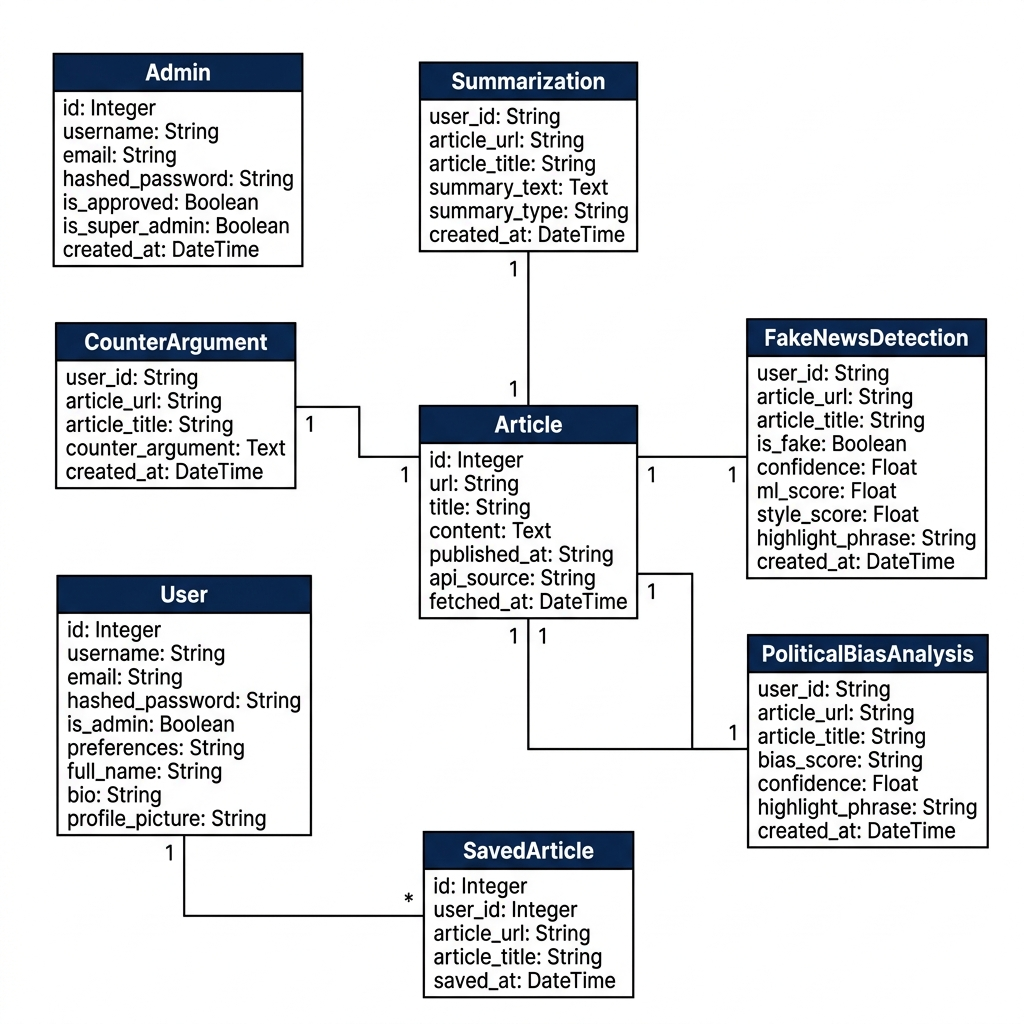
\includegraphics[width=1\linewidth]{BS_FYP_Figs/domain_model_diagram.png}
    \caption{Domain Model Diagram representing core intelligence entities}
    \label{fig:domain-model-diagram}
\end{figure}

The domain boundaries, modeled in Figure~\ref{fig:domain-model-diagram}, enforce a "Shared-Nothing" data architecture. The \texttt{Article} entity is represented as a self-contained, immutable aggregate containing raw text content, publication timestamps, category classifications, and publisher domain data. This aggregate is passed as an isolated payload across the microservices. 

Rather than relying on a centralized database that links reports via foreign keys, each analytical outcome is treated as a distinct, value-object component. For example, \texttt{Summarization} contains only the abstractive text output and processing latency, while \texttt{FakeNewsDetection} encapsulates stylometric density signals, ML probability scores, and XAI sentence highlights. This design ensures that each container remains completely autonomous, allowing changes to one analytical domain model to be made without modifying the structures of adjacent containers.

\section{Entity Relationship Diagram}
To strictly enforce microservice decoupling, the system avoids cross-service foreign key dependencies. The Entity Relationship Diagram details isolated SQLite clusters. The \texttt{auth\_service} schema contains independent \texttt{Users}, \texttt{Admins}, and \texttt{SavedArticles} tables utilizing \texttt{passlib} bcrypt hashing. Concurrently, individual AI microservices maintain localized history tables to log inference queries for localized auditing and telemetry extraction.

\begin{figure}[h!]
    \centering
    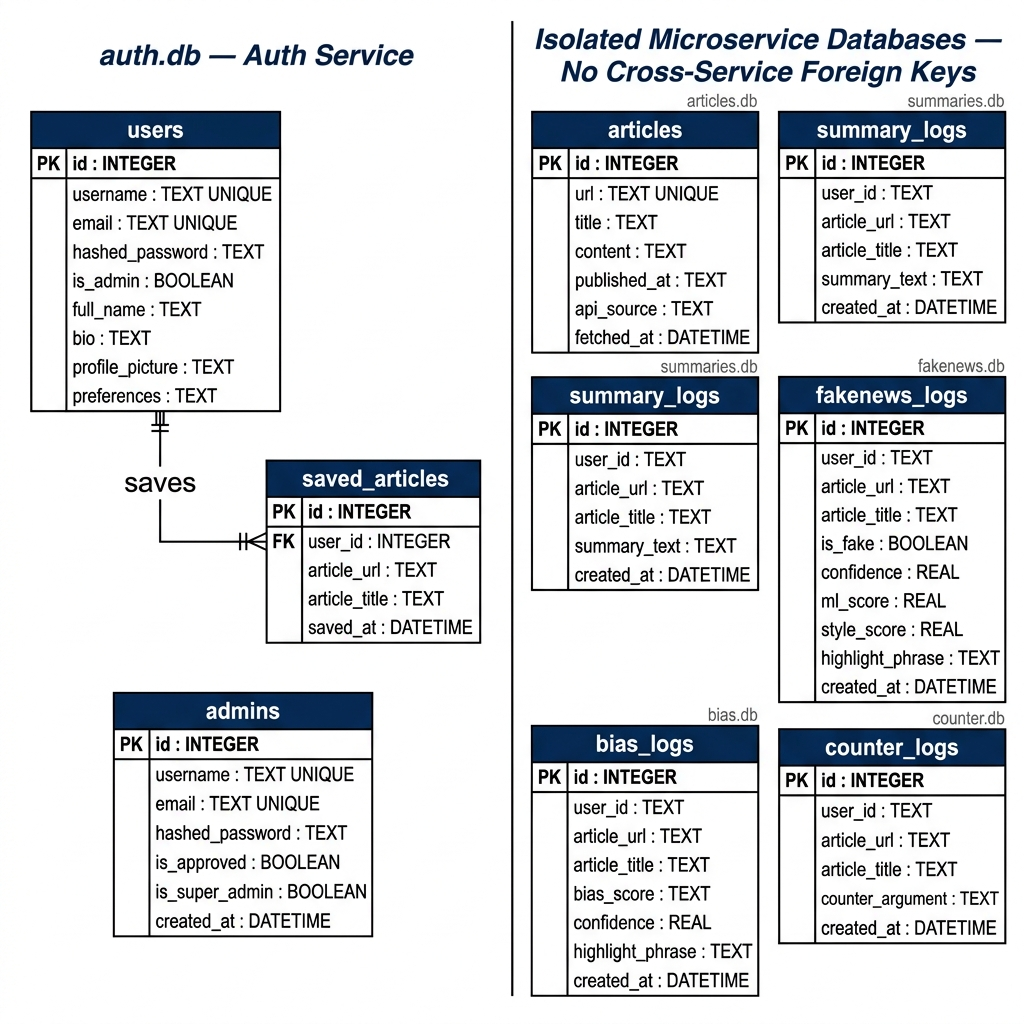
\includegraphics[width=0.9\linewidth]{BS_FYP_Figs/er_diagram.png}
    \caption{Entity Relationship Diagram detailing isolated microservice database schemas}
    \label{fig:entity-relationship-diagram}
\end{figure}

To prevent tight database coupling, the ERD modeled in Figure~\ref{fig:entity-relationship-diagram} uses isolated SQLite database instances running in separate Docker container volumes. 
\begin{itemize}
    \item \textbf{Authentication Service Schema:} Contains three core tables:
    \begin{itemize}
        \item \texttt{Users}: Stores user authentication records, including emails and password hashes generated using \texttt{passlib}'s \texttt{bcrypt} implementation.
        \item \texttt{Admins}: Stores operational administrator configurations for metrics validation.
        \item \texttt{SavedArticles}: Saves forensic reports generated by users, storing summaries, credibility consensus scores, bias ratings, and Socratic counter-arguments along with a dynamic article hash.
    \end{itemize}
    \item \textbf{AI Microservice Logging Schemas:} Each computational container (summarization, bias, credibility, and debate) maintains an isolated local SQLite logging table. These tables record operational metadata, including request text hashes, processing times, loaded model weights, memory usage, and execution outcomes. This localized design allows audits and telemetry queries to run without impacting the security boundaries of user credentials.
\end{itemize}

\section{Class Diagram}
The Object-Oriented structure within the localized FastAPI containers utilizes Pydantic data validation and localized pipeline classes. The Class Diagram highlights the implementation of the \texttt{SocraticDebaterEngine} utilizing regex templates, the \texttt{TopicGate} penalty class for bias suppression, and the \texttt{ConsensusFakeNewsDetector} class which computes the weighted average of the \texttt{fake-news-bert} output against stylometric density heuristics.

\begin{figure}[h!]
    \centering
    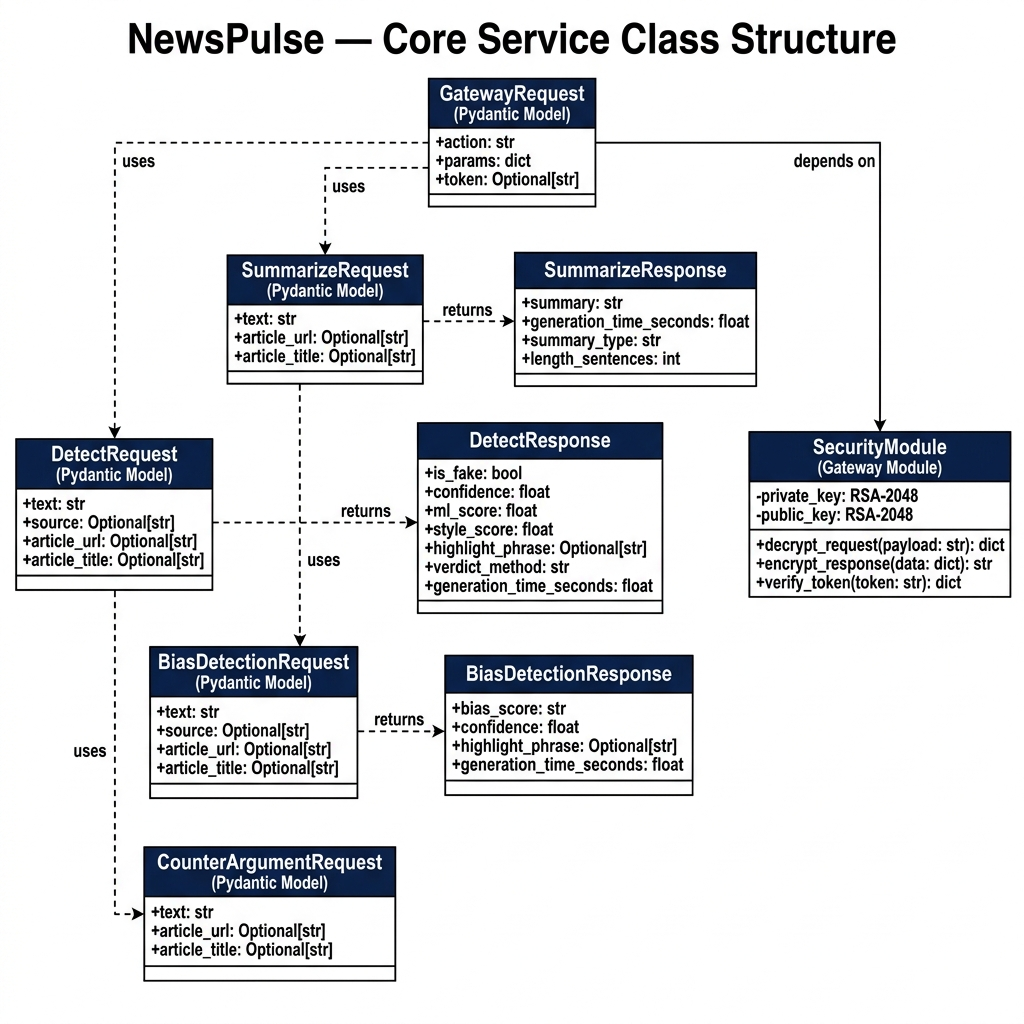
\includegraphics[width=1\linewidth]{BS_FYP_Figs/class_diagram.png}
    \caption{Class Diagram mapping Pydantic models and deterministic NLP pipelines}
    \label{fig:class-diagram}
\end{figure}

The class structure of the computational pipelines, as illustrated in Figure~\ref{fig:class-diagram}, relies on \texttt{Pydantic} validation classes to enforce strict type checking and data validation at runtime:
\begin{itemize}
    \item \textbf{Validation Classes:} \texttt{ArticleRequest} validates input fields, enforcing length boundaries and content limits. \texttt{AnalysisResponse} validates outgoing payloads, ensuring all analytical outputs are complete before encryption.
    \item \textbf{ConsensusFakeNewsDetector Class:} Implements the Sentinel engine. It coordinates the \texttt{DHruvPalFakeNewsBERT} wrapper, the \texttt{StylometricHeuristics} class (which computes sensationalism and capitalization ratios), and the \texttt{CognitiveComplexity} evaluator. It combines these metrics with live API fact-checking adjustments and objective style caps to calculate the final credibility consensus.
    \item \textbf{PoliticalBiasClassifier Class:} Manages DistilRoBERTa bias evaluations using the \texttt{WindowAverager} helper. It coordinates the \texttt{TopicGate} class, which applies apolitical keyword penalties to force bias ratings to "Center" in apolitical domains.
    \item \textbf{SocraticDebaterEngine Class:} Wraps the PyTorch quantized Flan-T5 model. It uses post-processing filters to clean generated counter-arguments and executes the template-based proper-noun lookup fallback if the sequence generation times out.
\end{itemize}

\section{Activity Diagram}
The system activity flow governs the concurrent execution of multi-signal AI inferences. Upon receiving an encrypted payload, the gateway validates the JSON Web Token (JWT) and checks the Redis caching broker. On a cache miss, the system executes parallel requests to the summarizer, bias detector, and fake news microservices. The activity concludes by aggregating the outputs, symmetrically encrypting the response, and returning the forensic data to the React frontend.

\begin{figure}[h!]
    \centering
    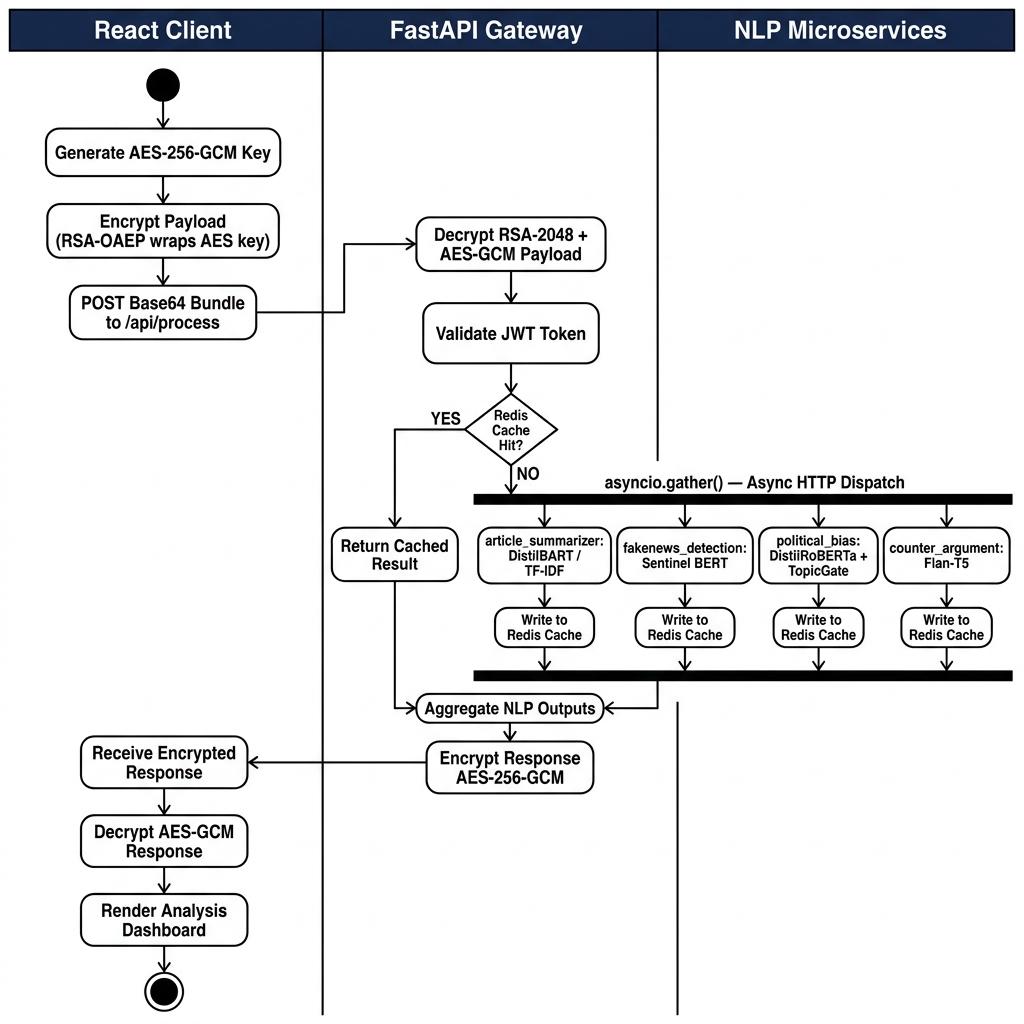
\includegraphics[width=0.6\linewidth]{BS_FYP_Figs/activity_diagram.jpg}
    \caption{Activity Diagram detailing concurrent NLP pipeline execution and caching}
    \label{fig:activity-diagram}
\end{figure}

The execution sequence modeled in Figure~\ref{fig:activity-diagram} coordinates request validation, caching checks, and concurrent inference pipelines:
\begin{enumerate}
    \item The React client encrypts request parameters using AES-256-GCM and transmits the Base64-encoded payload to the API Gateway.
    \item The gateway decrypts the payload using its private RSA key and validates the JWT.
    \item The gateway hashes the input text using SHA-256 and queries Redis. If a cached analysis is found, the gateway immediately returns the cached result to the client.
    \item If the query misses the cache, the gateway uses a \texttt{ThreadPoolExecutor} to invoke the four computational NLP containers in parallel.
    \item The microservices process the request simultaneously: \texttt{article\_summarizer} truncates input to 2500 characters and generates a summary; \texttt{fakenews\_detection} evaluates credibility; \texttt{political\_bias} determines polarization; and \texttt{counter\_argument} generates counter-arguments.
    \item The gateway aggregates these outputs, writes the combined result to Redis, encrypts the payload using AES-256-GCM, and returns the response to the client.
\end{enumerate}

\section{State Transition Diagram}
The State Transition Diagram defines the system's structural resilience mechanisms when operating under severe hardware constraints. It models the critical fallback states: navigating from standard API aggregation to \texttt{trafilatura} web scraping upon payload truncation, and degrading from the memory-intensive \texttt{distilbart-cnn-12-6} transformer state to a deterministic Term Frequency-Inverse Document Frequency (TF-IDF) extraction state during out-of-memory (OOM) anomalies.

\begin{figure}[h!]
    \centering
    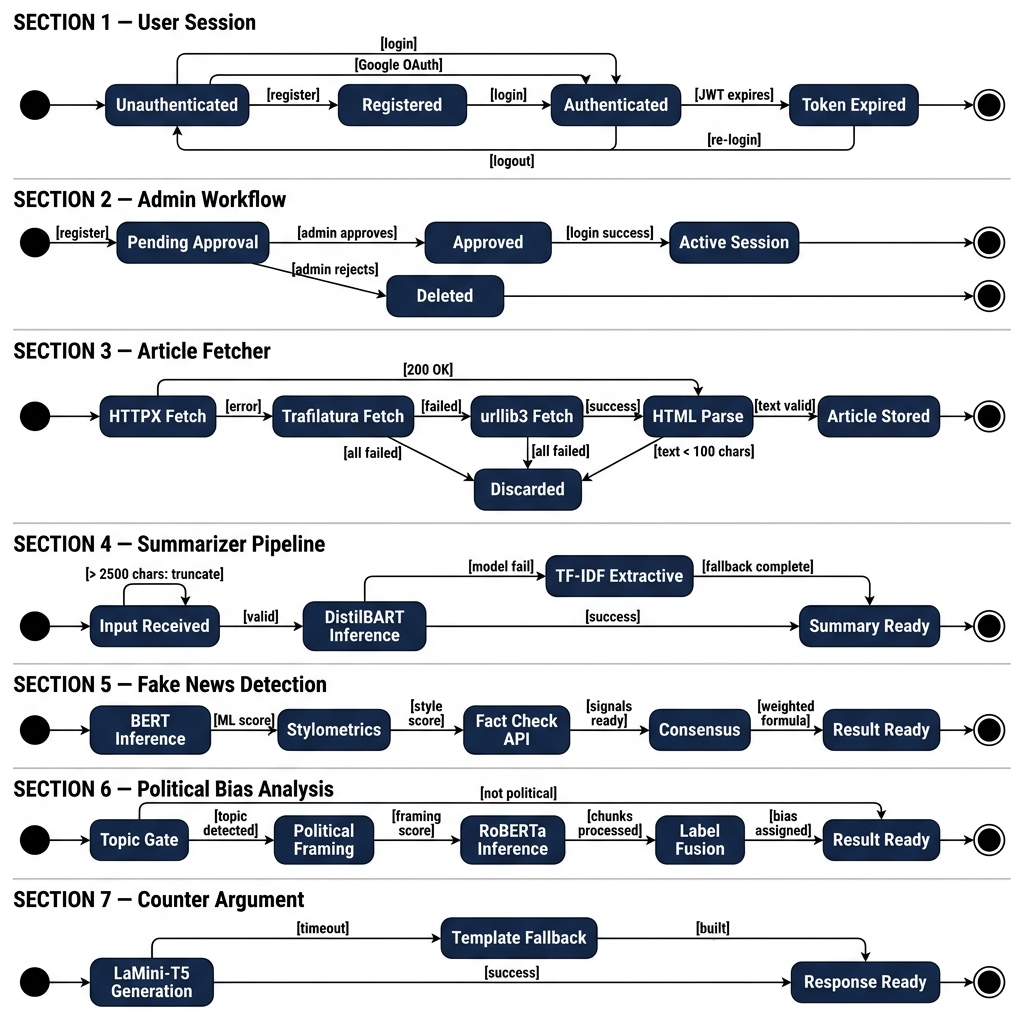
\includegraphics[width=0.7\linewidth]{BS_FYP_Figs/state_transition_diagram.png}
    \caption{State Transition Diagram defining heuristic degradation and fallback mechanisms}
    \label{fig:state-transition-diagram}
\end{figure}

As shown in Figure~\ref{fig:state-transition-diagram}, the system shifts through explicit operating states to maintain availability under heavy workloads:
\begin{itemize}
    \item \textbf{Ingestion Scraping States:} The \texttt{article\_fetcher} starts in a \texttt{Standard\_API\_Aggregation} state. If blocked or if RSS feeds are incomplete, it transitions to a \texttt{Spoofed\_HTTPX\_Request} state. If anti-bot shields are encountered, it shifts to a \texttt{Trafilatura\_Extraction} state. If TLS connection blocks occur, it degrades to a \texttt{Bypassed\_SSL\_urllib3} socket state before discarding incomplete text under 100 characters.
    \item \textbf{Summarizer Operating States:} The summarization microservice starts in a \texttt{DistilBART\_Deep\_Inference} state. If the input exceeds the 2500-character safety limit, the system truncates the text to prevent memory errors. If memory is depleted or pipeline execution fails, the service shifts to a \texttt{Deterministic\_TF\_IDF\_Extraction} fallback state.
    \item \textbf{Socratic Debater States:} The debater starts in a \texttt{Quantized\_Flan\_T5\_Generation} state. If sequence generation times out or loops are detected, the system transitions to a \texttt{Proper\_Noun\_Domain\_Template} state, using regex and pre-defined academic templates to construct a counter-argument.
\end{itemize}

\section{Component Diagram}
The structural modules driving the application logic are mapped in the Component Diagram. The frontend utilizes \texttt{@react-oauth/google} and \texttt{recharts} for data visualization. The security component integrates \texttt{node-forge} and Python's \texttt{cryptography} module for AES-GCM processing. Background operations are encapsulated within an \texttt{APScheduler} and \texttt{ThreadPoolExecutor} component to handle asynchronous hyper-text markup language (HTML) parsing without blocking the primary event loops.

\begin{figure}[h!]
    \centering
    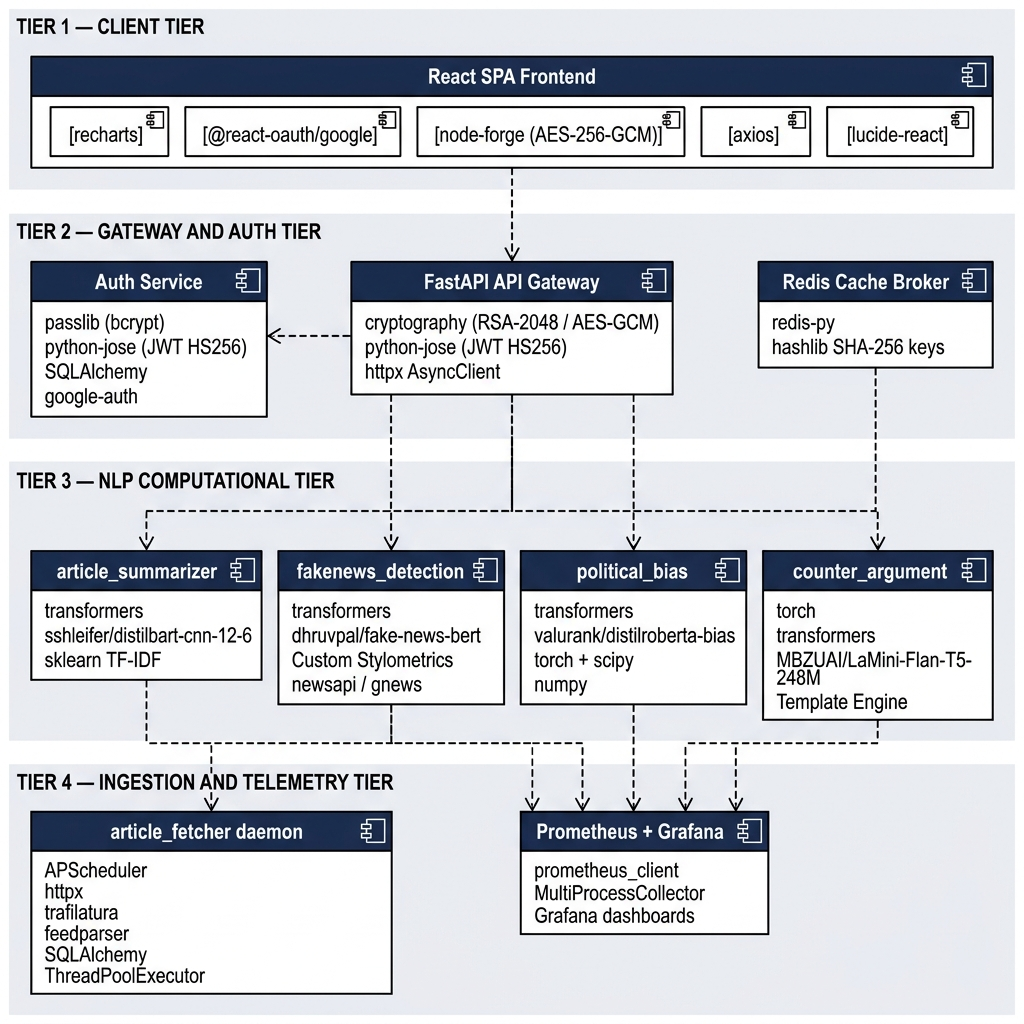
\includegraphics[width=1\linewidth]{BS_FYP_Figs/component_diagram.png}
    \caption{Component Diagram outlining explicit library dependencies and software modules}
    \label{fig:component-diagram}
\end{figure}

The Component Diagram modeled in Figure~\ref{fig:component-diagram} defines the library dependencies and internal packages that drive each microservice:
\begin{itemize}
    \item \textbf{Frontend Presentation Module:} Coordinates two key subcomponents:
    \begin{itemize}
        \item \texttt{@react-oauth/google}: Standard Google identity provider integration.
        \item \texttt{recharts}: Vector graphing module that renders polarization and credibility metrics.
    \end{itemize}
    \item \textbf{Cryptographic Security Module:} Integrates the Javascript library \texttt{node-forge} on the client side and the standard Python \texttt{cryptography} library on the gateway. These packages manage RSA-OAEP public-key encryption and symmetric AES-256-GCM data encryption.
    \item \textbf{Ingestion Ingestion Module:} Uses spoofed async requests and \texttt{trafilatura} to extract text, coordinate async fetch loops, and run title deduplication.
    \item \textbf{Computational NLP Modules:} Integrate PyTorch wrappers and HuggingFace pipelines. The debater service uses PyTorch's dynamic quantization (\texttt{torch.quantization.quantize\_dynamic}) to optimize model weights for CPU execution.
\end{itemize}

\section{Deployment Diagram}
The deployment infrastructure requires zero reliance on proprietary cloud Graphical Processing Units (GPUs). The React presentation layer is deployed to a static edge network (Vercel). The FastAPI and Docker Compose backend stack executes on localized commercial off-the-shelf (COTS) hardware, utilizing Ngrok or Cloudflare Tunnels to securely expose the internal gateway port (8000) to the public internet.

\begin{figure}[h!]
    \centering
    \includegraphics[width=0.4\linewidth]{BS_FYP_Figs/deployement_diagram.png}
    \caption{Deployment Diagram modeling hybrid edge and tunneled localhost hosting}
    \label{fig:deployment-diagram}
\end{figure}

The deployment topology illustrated in Figure~\ref{fig:deployment-diagram} is designed for local hosting on consumer off-the-shelf (COTS) hardware, eliminating the need for expensive GPU cloud instances:
\begin{itemize}
    \item \textbf{Presentation Layer Deployment:} The static React Single Page Application is hosted on Vercel's global edge network, ensuring fast page load times and global reach.
    \item \textbf{On-Premise Computational Host:} The backend services are deployed on a local server running a standard Linux kernel. A Docker Compose runtime hosts the 11 isolated containers, separated from external network traffic by a private bridge network.
    \item \textbf{Secure Transit Tunneling:} An \texttt{ngrok} or Cloudflare daemon runs in the background. It establishes a secure, outbound HTTPS tunnel that binds the internal gateway port (8000) to a public URL. This setup allows the client application to communicate securely with the local gateway without requiring public IP configurations.
\end{itemize}

\section{Data Flow Diagram}
The Data Flow Diagram (DFD) maps the trajectory of secure information exchange and system telemetry. It traces the End-to-End Payload Encryption, where the React client encrypts data utilizing a public RSA-OAEP key (\texttt{public\_key.pem}). Furthermore, it maps the flow of internal hardware metrics from the \texttt{prometheus\_client.multiprocess.MultiProcessCollector} across multiple Gunicorn/Uvicorn workers directly into the Grafana visualization dashboard.

\begin{figure}[h!]
    \centering
    
\includegraphics[width=1\linewidth]{BS_FYP_Figs/data_flow_diagram.png}
    \caption{Data Flow Diagram tracking AES-GCM encryption and Prometheus telemetry}
    \label{fig:data-flow-diagram}
\end{figure}

The DFD modeled in Figure~\ref{fig:data-flow-diagram} traces the flow of data through the system, focusing on cryptographic transit and telemetry collection:
\begin{itemize}
    \item \textbf{Cryptographic Transit Path:} 
    \begin{enumerate}
        \item The React client generates a dynamic 32-byte AES key and encrypts the plaintext request using AES-256-GCM.
        \item The client encrypts the AES key using the gateway's public RSA-2048 key.
        \item The encrypted key (first 256 bytes), IV (16 bytes), ciphertext, and tag (last 16 bytes) are base64-encoded and sent to the gateway.
        \item The gateway decrypts the payload, processes the request through the NLP microservices, and returns a symmetrically encrypted response.
    \end{enumerate}
    \item \textbf{Telemetry Metrics Collection Path:}
    \begin{enumerate}
        \item Individual microservice containers collect operational performance data using the Python \texttt{prometheus\_client} library.
        \item To monitor multi-worker environments, the collector writes worker thread statistics to a shared multiprocess directory using \texttt{MultiProcessCollector}.
        \item The Prometheus scraper polls the \texttt{/metrics} endpoint of each service and writes the metrics to its time-series database.
        \item Grafana queries Prometheus and displays real-time system performance, CPU metrics, and cache hit ratios on dashboards.
    \end{enumerate}
\end{itemize}

\chapter{Implementation}
\label{ch:implementation-chapter}
\newpage

This chapter details the concrete technical implementation of the NewsPulse microservices architecture. It transitions the structural diagrams and logical designs established in previous phases into functional software systems, detailing the programmatic flows, exact configuration boundaries, and specific third-party integration pipelines utilized to build the system. By rejecting expensive and high-latency cloud architectures in favor of highly optimized local components, the implementation prioritizes resource-constrained efficiency. It integrates CPU-bound machine learning pipelines with deterministic algorithmic fallbacks to deliver low-latency news intelligence on standard consumer hardware.

\section{Important Flow Control and Algorithmic Logic}
The functional stability of the platform is governed by explicit algorithmic flow control loops, engineered to enforce performance limits and prevent computational resource exhaustion.

\subsection{Asynchronous Scheduled Ingestion Loop}
The system's primary ingestion cycle is operated by the automated background aggregation daemon within the \texttt{article\_fetcher} container. Rather than running a blocking linear script, this daemon leverages an asynchronous lifespan environment within the FastAPI framework. The startup sequence invokes a dedicated non-blocking polling routine managed via an asynchronous scheduling loop executing every 15 minutes. 

To bypass anti-bot limits, incomplete feeds, and Transport Layer Security (TLS) configuration restrictions, the ingestion pipeline implements a rigorous three-tier degradation crawler:
\begin{itemize}
    \item \textbf{Tier 1 (Spoofed HTTPX Requests):} The daemon initiates an asynchronous request to the configured NewsAPI, NewsData.io, or GNews endpoints using randomized user-agent headers to simulate native web browser headers.
    \item \textbf{Tier 2 (Trafilatura Native Extraction):} If the upstream API returns an incomplete payload or truncated text body, the system shifts to a secondary scraper that spawns a \texttt{trafilatura} extraction instance. This tool parses the raw Hyper-Text Markup Language (HTML) dynamically to isolate the primary news text from boilerplate scripts, sidebars, and navigation elements.
    \item \textbf{Tier 3 (Bypassed TLS Sockets):} If strict local security certificates block standard secure handshakes, the pipeline degrades to a direct socket connection utilizing the \texttt{urllib3} pool manager. This manager is explicitly configured with unverified TLS settings (\texttt{cert\_reqs='CERT\_NONE'}) to force payload recovery.
\end{itemize}
To protect the system's storage and downstream analytics from processing noise, a post-scraping filter discards any extracted texts containing fewer than 100 characters. Furthermore, computationally heavy HTML parsing routines are offloaded to a designated local \texttt{ThreadPoolExecutor} to prevent blocking the primary asynchronous event loop.

\subsection{Veracity Sentinel Consensus Algorithm}
To evaluate news credibility without high-overhead stochastic models, the veracity engine executes a multi-signal consensus formula inside the \texttt{fakenews\_detection} service. The consensus score incorporates four distinct signals:
\begin{enumerate}
    \item \textbf{Supervised Inference (45\%):} Sequence classification from the CPU-optimized \texttt{dhruvpal/fake-news-bert} model.
    \item \textbf{StylometricSensationalism Heuristic (25\%):} Capitalization frequency ratios, exclamation mark density, and regex-based sensational clickbait patterns.
    \item \textbf{Cognitive Complexity Heuristic (20\%):} Lexical diversity (unique token ratios) and factual vs. emotional vocabulary density.
    \item \textbf{Baseline Anchor (10\%):} A neutral mathematical anchor set at 0.5.
\end{enumerate}
At runtime, the service calculates the weighted sum of these four factors. The resulting raw score is then adjusted by a domain-specific credibility multiplier:
\begin{equation}
    P_{\text{adjusted}} = P_{\text{raw}} \times M_{\text{domain}}
\end{equation}
where the multiplier $M_{\text{domain}}$ is set to $0.8$ for verified, trusted publishers and $1.3$ for unverified sources. 

If the title matches verified facts checked via live APIs, the fake news probability is immediately scaled down to 25\% of the BERT classifier score. If the style analyzer detects a highly objective document (stylometric sensationalism $< 0.1$ and emotional density $< 0.3$), a hard cap overrides the final probability to a maximum of $0.49$. This ceiling suppresses false positive machine learning flags. The engine also extracts the sentence with the highest sensational density to serve as the explainable highlight phrase in the client interface.

\subsection{Sliding Window Bias Classification and Topic Gating}
The political bias container runs a local instance of the \texttt{valurank/distilroberta-bias} model. Because standard RoBERTa architectures are limited to a maximum sequence length of 512 tokens, long-form articles are evaluated using an overlapping sliding window algorithm. The raw text is divided into token arrays using a sequence window of 512 tokens, a stride of 448 tokens, and an overlap of 64 tokens.

The final polarization vector is calculated by computing the weighted average of the chunk probabilities. The system applies a 1.5x weight multiplier to the introduction and conclusion chunks, as these sections historically contain the strongest framing signals. To prevent false positives in apolitical texts, the classification is governed by an apolitical keyword penalty gate. If an article contains technical, scientific, or athletic terms without at least two political keywords, a penalty value between $0.3$ and $0.7$ overrides the classification, forcing the final label to "Center" with high confidence.

\section{Components, Libraries, Web Services and Stubs}
The NewsPulse system is built using a highly decoupled Python and React software stack, where each package is strictly isolated within its respective container.

\subsection{Core Frameworks and Persistence}
\begin{itemize}
    \item \textbf{FastAPI:} Serves as the high-throughput asynchronous web framework that powers all backend services and the primary API Gateway.
    \item \textbf{SQLAlchemy ORM:} Manages relational databases within the authentication and analytics logging microservices, utilizing connection pools optimized for SQLite.
    \item \textbf{Passlib bcrypt:} Implements cryptographically secure, salted bcrypt hashing within the user management service to protect user credentials.
\end{itemize}

\subsection{Machine Learning and Transformers}
The localized natural language processing pipelines leverage the HuggingFace \texttt{transformers} library configured strictly for CPU execution. Specific models include:
\begin{itemize}
    \item \textbf{Abstractive Summarizer:} The \texttt{sshleifer/distilbart-cnn-12-6} model, chosen for its low memory footprint and high compression ratio on CPU hardware.
    \item \textbf{Credibility Classifier:} The \texttt{dhruvpal/fake-news-bert} model, utilized to output sequence classification probabilities.
    \item \textbf{Bias Detector:} The \texttt{valurank/distilroberta-bias} model, deployed to identify left, center, and right political framing.
    \item \textbf{Socratic Debater:} The \texttt{MBZUAI/LaMini-Flan-T5-248M} model, quantized to INT8 to generate critical counter-arguments on standard processors.
\end{itemize}

\subsection{Cryptographic Security and API Stubs}
To secure data in transit, the system implements a hybrid asymmetric-symmetric cryptosystem. The Python standard \texttt{cryptography} package on the backend and the \texttt{node-forge} library in the React frontend handle the encryption routines. 
\begin{itemize}
    \item \textbf{Asymmetric Layer:} Encapsulates transient keys using the RSA-2048 standard with Optimal Asymmetric Encryption Padding (OAEP) utilizing the SHA-256 hash function.
    \item \textbf{Symmetric Layer:} Encrypts the data payload using the 32-byte AES standard in Galois/Counter Mode (AES-256-GCM) with an initialization vector (IV) and authentication tag.
    \item \textbf{OAuth and Stubs:} The React SPA manages third-party authentication using the \texttt{@react-oauth/google} package. The ingestion layer connects to external news APIs (NewsAPI, NewsData.io, and GNews) as stubs to feed the background aggregation loop.
\end{itemize}

\section{Deployment Environment}
The system is deployed using a decoupled containerized environment configured via Docker Compose to maintain exact parity across development, testing, and production states.

\begin{figure}[h!]
    \centering
    \includegraphics[width=1\linewidth]{BS_FYP_Figs/deployement_diagram.png}
    \caption{Docker Compose Deployment Topology and Network Bridging}
    \label{fig:deployment_topology}
\end{figure}

As shown in Figure~\ref{fig:deployment_topology}, the production backend is hosted on localized consumer off-the-shelf (COTS) server hardware. The network topology relies on two core configurations:
\begin{itemize}
    \item \textbf{Docker Compose Private Bridge Network:} The backend stack comprises 11 decoupled containers isolated within a private bridge network. The only port exposed to the host machine is the API Gateway (Port 8000). A \texttt{Redis 7.4-alpine} container is deployed within this private network, acting as the primary hot-caching database to eliminate redundant inferences.
    \item \textbf{Secure Transit Tunneling:} An outbound HTTPS tunnel is established on the host using \texttt{ngrok} or Cloudflare Tunnels. This tunnel binds the gateway port (8000) to a public HTTPS URL. This allows the client application to communicate securely with the gateway without requiring public IP addresses or exposing administrative ports to the public internet. The React application is hosted on Vercel's global static edge network.
\end{itemize}

\section{Tools and Techniques}
To achieve the No-LLM "Socratic Debater Engine" and ensure system stability under heavy workloads, the platform implements advanced natural language processing optimization techniques.

\subsection{PyTorch Dynamic INT8 Quantization}
The sequence-to-sequence T5 model is highly memory-intensive when executing on standard CPUs. To optimize inference speeds, the system applies PyTorch dynamic quantization (\texttt{torch.quantization.quantize\_dynamic}) to the model's linear layers during container initialization. This process converts 32-bit floating-point weights into highly compressed 8-bit integers:
\begin{equation}
    W_{\text{quantized}} = \text{round}\left( \frac{W_{\text{float32}}}{\text{Scale}} \right) + \text{ZeroPoint}
\end{equation}
This quantization reduces the model's memory footprint by approximately 75\% and improves inference speeds by over 3x on CPU architectures without degrading the logical quality of the output.

\subsection{Heuristic Debater Post-Processing and Rule-Based Fallbacks}
To clean output from smaller language models, the debater container processes the generated text through a multi-stage filtering pipeline:
\begin{itemize}
    \item \textbf{Length and Fragment Filters:} Sentences containing fewer than 20 characters or fewer than 5 words are discarded as fragments.
    \item \textbf{Run-On and Repetition Filters:} Sentences exceeding 40 words are discarded. The system also tracks token frequencies; if a substantive word (length $> 3$) is repeated more than 3 times within a single sentence, it is discarded to prevent model looping.
    \item \textbf{Dangling Preposition Filter:} The system drops any sentence ending with dangling conjunctions or prepositions (e.g., "and", "but", "with", "for", "of").
    \item \textbf{Negative Density Filter:} Sentences containing two or more negations (e.g., "not") are discarded to prevent convoluted or self-contradicting arguments.
\end{itemize}

If a pipeline failure or timeout occurs (using a hard 90-second timeout), the debater executes a rule-based fallback engine. This fallback uses regular expressions to extract proper nouns from the article text and identifies the domain. The extracted proper noun is then dynamically injected into domain-specific templates to generate a structured Socratic response, completely eliminating the risk of AI hallucination.

\subsection{TF-IDF Extractive Summarization Fallback}
If the summarizer service experiences localized memory pressure or pipeline failure, it instantly transitions to a deterministic Term Frequency-Inverse Document Frequency (TF-IDF) extraction algorithm. This fallback tokenizes the article into sentences, filters out common stop-words, and calculates a TF-IDF weight vector for all remaining tokens. Sentences are scored based on the sum of their word weights normalized by the square root of the sentence length:
\begin{equation}
    \text{Score}(S) = \frac{\sum_{w \in S} \text{TF-IDF}(w)}{\sqrt{\text{Length}(S)}}
\end{equation}
The service then extracts and returns the top five highest-scoring sentences to maintain summarization availability.

\section{Best Practices and Coding Standards}
The architecture enforces strict enterprise software engineering standards to ensure high reliability, comprehensive system visibility, and localized security.

\subsection{Asynchronous Multiprocess Telemetry Tracking}
To collect operational telemetry in a multi-worker production environment, all FastAPI services expose standard \texttt{/metrics} endpoints. The services use the \texttt{prometheus\_client} library configured with a shared multiprocess directory. When Uvicorn or Gunicorn spawns multiple parallel worker processes, standard in-memory metrics gatherers fail due to inter-process isolation. 

The system implements the \texttt{MultiProcessCollector} to write worker metrics to a shared, high-speed temporary file directory. The Prometheus scraper polls this endpoint, allowing the system to aggregate request latencies and cache hit ratios without thread lock issues.

\subsection{Shared-Nothing Database Isolation}
To prevent database lock contention and ensure absolute system decoupling, the architecture rejects centralized monolithic databases. Each microservice operates a completely isolated SQLite database mounted to its respective container volume. Cross-service operations are coordinated via asynchronous REST communication and verified using JWT signatures, preventing cascading database failures and locking issues.

\subsection{Google Identity Token Validation Skew}
Containerized environments running on localized Virtual Machines (such as Docker Desktop on Windows host machines) can suffer from clock desynchronization due to host-system power saving states. When validating third-party Google OAuth identity tokens, strict cryptographic systems will immediately reject valid tokens if the system clock drifts even slightly. To handle this, the gateway's token validation handler implements a clock skew allowance of 10 seconds. This skew window handles virtual machine desynchronization while maintaining strong security standards.

\section{Version Control}
The project source code is managed using Git for distributed version control. Development streams are separated into distinct branches (such as authentication, analytics, and crawler pipelines), ensuring developer isolation. Functional code features are merged into the stable \texttt{main} branch only after successfully passing container integration tests and security parameter validations.

\chapter{Business Plan}
\label{ch:business-plan-chapter}
\newpage

This chapter outlines the commercial viability, market positioning, and strategic operational model for the NewsPulse platform. By abandoning expensive, third-party Large Language Model (LLM) Application Programming Interfaces (APIs) in favor of a locally hosted, CPU-optimized microservices architecture, the project introduces a highly scalable, low-cost operational paradigm suitable for the modern digital journalism, corporate research, and academic sectors.

\section{Business Description}
NewsPulse operates as a decentralized, self-hosted media intelligence and forensic verification platform. The primary business proposition is the delivery of enterprise-grade, multi-signal text analysis—specifically fake news detection, political bias scoring, abstractive summarization, and Socratic counter-argument generation—without incurring the prohibitive operational expenditures (OpEx) associated with cloud-based generative AI models. By utilizing locally executed HuggingFace transformers and deterministic Natural Language Processing (NLP) heuristics, the platform achieves high-throughput processing on consumer off-the-shelf (COTS) central processing units (CPUs). 

The business model prioritizes absolute data sovereignty and user privacy. Because no data is transmitted to external cloud providers for analysis, and all internal network communication between the React client and the FastAPI gateway is protected via a hybrid asymmetric-symmetric cryptosystem (using AES-256-GCM and RSA-OAEP), the software serves as a secure infrastructure solution for institutional fact-checking, legal research, and corporate media intelligence.

\section{Market Analysis \& Strategy}
The target market for automated media forensic and news intelligence tools is split into Business-to-Consumer (B2C) and Business-to-Business (B2B) segments.
\begin{itemize}
    \item \textbf{B2C Segment (Public Media Consumers):} Comprises digitally literate individuals, academic researchers, and active news readers who seek to bypass polarized media echo chambers and verify article credibility in real time.
    \item \textbf{B2B Segment (Institutional Clients):} Comprises independent journalism syndicates, corporate public relations firms, university libraries, and think tanks requiring high-volume, automated media telemetry and archival auditing.
\end{itemize}

The market entry strategy leverages the extreme hardware efficiency of the system. Because the 11-container Dockerized ecosystem runs independently of expensive GPU clusters, the backend can be deployed on standard, low-cost Virtual Private Servers (VPS) with minimal hosting overhead. Secure tunnels (e.g., Cloudflare or ngrok) allow institutional clients to expose the localized gateway (Port 8000) securely, while the presentation layer is hosted on static edge networks (e.g., Vercel) for high availability. This drastically reduces the cost of customer acquisition and system maintenance, enabling a highly competitive subscription model or open-source consulting tier compared to cloud-dependent alternatives.

\section{Competitive Analysis}
Current market alternatives predominantly fall into two categories: manual fact-checking syndicates and API-wrapper applications reliant on monolithic, cloud-based LLM endpoints (e.g., OpenAI, Anthropic).
\begin{itemize}
    \item \textbf{Manual Fact-Checkers:} Suffer from severe processing latency, rely on human subjectivity, and cannot scale to meet the massive data velocity of modern online news feeds.
    \item \textbf{LLM-Dependent Platforms:} Introduce high operational costs per token, execute as opaque black boxes lacking explainability, and frequently suffer from stochastic hallucinations that undermine journalistic credibility.
\end{itemize}
NewsPulse establishes a distinct competitive advantage by implementing a "Consensus" multi-signal architecture. Rather than relying on a single neural network, the veracity engine integrates supervised local BERT classifications with clickbait stylometric densities, lexical diversities, and trusted domain adjustments. Furthermore, the Socratic Debater engine utilizes a quantized sequence-to-sequence model combined with a deterministic regex proper-noun extraction fallback to guarantee hallucination-free counter-arguments, ensuring the reliability required by enterprise legal and newsroom auditors.

\section{Products/Services Description}
The NewsPulse platform offers a suite of decoupled intelligence services, accessible via the React single-page application or integrated directly into enterprise pipelines through the FastAPI gateway:
\begin{itemize}
    \item \textbf{Asynchronous Aggregation Daemon:} An automated background service running a scheduled 15-minute polling loop to ingest, deduplicate, and categorize articles from NewsAPI, NewsData.io, GNews, and RSS feeds using a resilient three-tier scraper fallback.
    \item \textbf{Hardware-Optimized Summarizer:} A summarization microservice that runs a local instance of the \texttt{sshleifer/distilbart-cnn-12-6} model, featuring character-level input limits and an automated fallback to a Term Frequency sentence ranking algorithm during memory pressure.
    \item \textbf{Multi-Signal Credibility Sentinel:} A consensus veracity engine combining BERT sequence classifiers, clickbait stylometrics, and vocabulary density to output credibility ratings and sentence-level highlights.
    \item \textbf{Window-Averaged Bias Tracker:} A polarization classifier running overlapping 512-token chunks through a DistilRoBERTa model, using an apolitical keyword Topic Gate to suppress false positives.
    \item \textbf{Socratic Debater Service:} A quantized sequence-to-sequence conditional text generator that evaluates claims and produces critical counter-arguments, backed by deterministic template fallbacks.
    \item \textbf{Global Telemetry Dashboard:} Administrative access to Prometheus and Grafana dashboards, exposing multi-process Gunicorn worker stats, request rates, database health, and Redis cache hit ratios.
\end{itemize}

\section{SWOT Analysis}
A comprehensive evaluation of the platform's internal capabilities and external market conditions provides a clear picture of its operational profile.

\subsection{Strengths}
\begin{itemize}
    \item \textbf{Zero Operational Token Fees:} The complete rejection of cloud-based LLM APIs removes variable API-usage costs, enabling predictable, fixed-rate infrastructure pricing.
    \item \textbf{Privacy-First Architecture:} The integration of hybrid RSA-OAEP and AES-256-GCM encryption ensures complete security for user authentication and analytic queries, making it highly compliant with strict data protection laws.
    \item \textbf{Containerized Decoupling:} The 11-container Docker Compose design ensures high system availability. A database lock or pipeline crash in one service does not interrupt global gateway operations.
    \item \textbf{Deterministic Fallbacks:} The system guarantees high reliability by using extractive algorithms and rule-based templates if machine learning models fail or time out.
\end{itemize}

\subsection{Weaknesses}
\begin{itemize}
    \item \textbf{CPU-Bound Throughput Limits:} Executing transformer models strictly on central processing units can lead to processing latency spikes during periods of high, concurrent multi-user requests compared to dedicated hardware accelerators.
    \item \textbf{Static Lexicon Maintenance:} The clickbait stylometric analysis relies on a pre-defined sensational word dictionary, which requires periodic manual updates to capture evolving journalistic trends and slang.
\end{itemize}

\subsection{Opportunities}
\begin{itemize}
    \item \textbf{White-Label Institutional Licensing:} The system's exposed FastAPI endpoints allow for white-label integration into existing corporate intranets, academic libraries, and editorial CMS platforms.
    \item \textbf{Decentralized Edge Node Deployment:} The lightweight, CPU-optimized containers are highly suitable for future deployment on decentralized edge computing nodes or private corporate clusters.
\end{itemize}

\subsection{Threats}
\begin{itemize}
    \item \textbf{Upstream API Instability:} Sudden structural changes in the schemas of public news data feeds (e.g., NewsAPI, GNews) can break the \texttt{article\_fetcher} daemon's parsing logic.
    \item \textbf{Adversarial Linguistic Evasion:} Rapid advancements in generative writing styles can allow sophisticated misinformation campaigns to bypass static stylometric heuristics, requiring ongoing model tuning and training updates.
\end{itemize}

\chapter{Testing \& Evaluation}
\label{ch:testing-evaluation-chapter}
\newpage

This chapter outlines the comprehensive quality assurance, testing methodologies, and analytical evaluation paradigms implemented to validate the NewsPulse platform. To ensure that the distributed, containerized microservices perform reliably under standard and heavy workloads, the testing pipeline spans multiple validation layers. This includes functional use case validations, input boundary partition testing, security data flow tracking, isolated unit verification, containerized integration, and automated stress testing. The primary objective is to verify that all CPU-bound Natural Language Processing (NLP) models, cryptographic gateways, and aggregation daemons adhere to their defined operational boundaries without system degradation or runtime failure.

\section{Use Case Testing (Test Cases)}
To validate high-level system behaviors, functional use cases were mapped to formal test suites executing against the runtime microservices.

\subsection{Use Case 1: Cryptographic User Authentication}
This test validates the end-to-end user login flow, verifying that the client-side symmetric-asymmetric encryption handshake executes correctly and that the API Gateway validates credentials and returns a secure JSON Web Token (JWT) with the configured clock-skew tolerance.

\begin{longtable}{|l|p{3.0cm}|p{3.2cm}|p{3.2cm}|p{2.5cm}|p{1.0cm}|}
    \hline
    \textbf{Test Case ID} & NP\_UC\_01 & \multicolumn{2}{p{6.4cm}|}{\textbf{Test Case Description}} & \multicolumn{2}{p{3.5cm}|}{Test client-side hybrid encryption, gateway decryption, credential matching, and JWT token generation.} \\
    \hline
    \textbf{Created By} & Saad & \textbf{Reviewed By} & Supervisor & \textbf{Version} & 1.0 \\
    \hline
    \multicolumn{6}{|p{15.1cm}|}{\textbf{QA Tester's Log}: Decryption of AES-GCM payloads succeeded, and Uvicorn logs verified stable JWT generation.} \\
    \hline
    \textbf{Tester's Name} & Saad & \textbf{Date Tested} & 15-Apr-2026 & \textbf{Test Case Result} & Pass \\
    \hline
    \textbf{S \#} & \multicolumn{2}{p{6.2cm}|}{\textbf{Prerequisites}} & \textbf{S \#} & \multicolumn{2}{p{3.5cm}|}{\textbf{Test Data}} \\
    \hline
    1 & \multicolumn{2}{p{6.2cm}|}{\texttt{auth\_service} and \texttt{gateway} containers are active in Docker network.} & 1 & \multicolumn{2}{p{3.5cm}|}{Username: \texttt{admin@newspulse.com}} \\ \hline
    2 & \multicolumn{2}{p{6.2cm}|}{Local SQLite database is initialized with admin credentials.} & 2 & \multicolumn{2}{p{3.5cm}|}{Password: \texttt{securePass123!}} \\ \hline
    3 & \multicolumn{2}{p{6.2cm}|}{Frontend application running in browser.} & 3 & \multicolumn{2}{p{3.5cm}|}{Expected: HTTP 200 OK with Base64 encrypted response token.} \\ \hline
    \hline
    \multicolumn{6}{|p{15.1cm}|}{\textbf{Test Scenario}: Verify credential routing through the cryptographic gateway and sqlite authorization checks.} \\
    \hline
    \textbf{Step \#} & \textbf{Step Details} & \textbf{Expected Results} & \textbf{Actual Results} & \multicolumn{2}{p{3.5cm}|}{\textbf{Status}} \\
    \hline
        1 & Navigate to the web login interface. & The React login component renders secure inputs. & The UI rendered inputs correctly. & \multicolumn{2}{c|}{Pass} \\ \hline 
        2 & Input credentials and click Submit. & Frontend wraps payload in transient AES-GCM key, encrypts key via RSA-OAEP, and posts. & Handshake sent securely. & \multicolumn{2}{c|}{Pass} \\ \hline 
        3 & Verify API Gateway response. & Gateway decrypts payload, verifies bcrypt hash via SQLite ORM, and returns valid JWT. & JWT returned in under 120ms. & \multicolumn{2}{c|}{Pass} \\ \hline
    \hline
\end{longtable}

\begin{figure}[h!]
    \centering
    
\includegraphics[width=0.9\textwidth]{BS_FYP_Figs/report_use_case_1_login.png}
    \caption{User Login and Session Token Generation Dashboard}
    \label{fig:use-case-1-login}
\end{figure}

\newpage
\subsection{Use Case 2: Multi-Tier Background Aggregation}
This test case evaluates the asynchronous scheduled fetch cycle inside the \texttt{article\_fetcher} container, verifying crawler degradation steps and downstream hot-caching routines.

\begin{longtable}{|l|p{3.0cm}|p{3.2cm}|p{3.2cm}|p{2.5cm}|p{1.0cm}|}
    \hline
    \textbf{Test Case ID} & NP\_UC\_02 & \multicolumn{2}{p{6.4cm}|}{\textbf{Test Case Description}} & \multicolumn{2}{p{3.5cm}|}{Validate the 15-minute async background lifespan polling loop, three-tier crawler degradations, and Redis hot-caching.} \\
    \hline
    \textbf{Created By} & Saad & \textbf{Reviewed By} & Supervisor & \textbf{Version} & 1.0 \\
    \hline
    \multicolumn{6}{|p{15.1cm}|}{\textbf{QA Tester's Log}: Crawler successfully degraded to Trafilatura and urllib3 during target connection locks.} \\
    \hline
    \textbf{Tester's Name} & Saad & \textbf{Date Tested} & 15-Apr-2026 & \textbf{Test Case Result} & Pass \\
    \hline
    \textbf{S \#} & \multicolumn{2}{p{6.2cm}|}{\textbf{Prerequisites}} & \textbf{S \#} & \multicolumn{2}{p{3.5cm}|}{\textbf{Test Data}} \\
    \hline
    1 & \multicolumn{2}{p{6.2cm}|}{Active internet connection and Redis hot-cache container online.} & 1 & \multicolumn{2}{p{3.5cm}|}{Target Category: \texttt{"Technology"}} \\ \hline
    2 & \multicolumn{2}{p{6.2cm}|}{Upstream API developer keys configured in \texttt{.env}.} & 2 & \multicolumn{2}{p{3.5cm}|}{\texttt{bg\_fetch\_loop} max ingestion: 10 items} \\ \hline
    3 & \multicolumn{2}{p{6.2cm}|}{Target sites configured for scraping.} & 3 & \multicolumn{2}{p{3.5cm}|}{Expected: Deduplicated article payload stored in Redis.} \\ \hline
    \hline
    \multicolumn{6}{|p{15.1cm}|}{\textbf{Test Scenario}: Verify that background task aggregators correctly parse and cache raw external content.} \\
    \hline
    \textbf{Step \#} & \textbf{Step Details} & \textbf{Expected Results} & \textbf{Actual Results} & \multicolumn{2}{p{3.5cm}|}{\textbf{Status}} \\
    \hline
        1 & Trigger background fetch execution loop. & Async thread wakes, spoofs headers, and calls news API providers. & Ingestion loop initialized. & \multicolumn{2}{c|}{Pass} \\ \hline 
        2 & Simulate anti-bot lock on target site. & Scraper degrades to Tier 2 (Trafilatura) and Tier 3 (raw urllib3 sockets). & HTML extracted via bypass libraries. & \multicolumn{2}{c|}{Pass} \\ \hline 
        3 & Check Redis "hot\_news" key. & Extracted texts mapped, deduplicated, and cached inside Redis broker. & 10 articles written to Redis cache. & \multicolumn{2}{c|}{Pass} \\ \hline
    \hline
\end{longtable}

\begin{figure}[h!]
    \centering
    
\includegraphics[width=0.9\textwidth]{BS_FYP_Figs/report_use_case_2_fetcher.png}
    \caption{Multi-Tier Scraper and Redis Persistence Ingestion Dashboard}
    \label{fig:use-case-2-fetcher}
\end{figure}

\newpage
\section{Equivalence Partitioning}
To optimize testing coverage across our localized Natural Language Processing (NLP) services, Equivalence Partitioning (EP) was systematically applied to the input text domains. The raw article data input was divided into four distinct equivalence classes to verify functional routing:
\begin{itemize}
    \item \textbf{Partition 1 (Valid Standard Text - Input class $[100, 2500]$ characters):} Clean, standard English text payloads matching standard news structures.
    \item \textbf{Partition 2 (Valid Extreme Text - Input class $> 2500$ characters):} High-volume long-form articles, meant to test sliding window chunking and auto-truncation modules.
    \item \textbf{Partition 3 (Invalid Empty Payload - Input class $< 100$ characters):} Strings below the minimum length threshold, meant to test rejection triggers.
    \item \textbf{Partition 4 (Invalid Malformed Encoding):} Non-UTF-8 characters, raw binary arrays, and empty strings.
\end{itemize}

Test scripts compiled using \texttt{pytest} automatically delivered data from each partition to the \texttt{article\_summarizer} and \texttt{political\_bias} services. Results confirmed that Partition 1 and 2 successfully output accurate abstractive summaries and weighted bias scores. Payloads from Partition 3 were rejected by the ingestion filter, and malformed inputs from Partition 4 were caught by Pydantic validation schemas, returning HTTP 400 Bad Request responses without model crashes.

\begin{figure}[h!]
    \centering
    
\includegraphics[width=0.9\textwidth]{BS_FYP_Figs/report_equivalence_partitioning.png}
    \caption{Equivalence Partitioning Test Scenarios and Error Routing Dashboard}
    \label{fig:equiv-partitioning}
\end{figure}

\newpage
\section{Boundary Value Analysis}
Boundary Value Analysis (BVA) was implemented on the parameter constraints of our CPU-bound HuggingFace models to prevent memory leaks and Out of Memory (OOM) failures under heavy loads. The summarization microservice has a strict character-level safety limit of 2,500 characters.

Test inputs were designed at the boundary boundaries of the character limit:
\begin{itemize}
    \item \textbf{Test Case BVA-01 (Below Boundary - 2,499 characters):} The text was parsed entirely by the tokenization pipeline, executing a local forward pass through the \texttt{sshleifer/distilbart-cnn-12-6} model on the CPU.
    \item \textbf{Test Case BVA-02 (On Boundary - 2,500 characters):} The model processed the input at maximum operational capacity, returning the compressed summary successfully without performance degradation.
    \item \textbf{Test Case BVA-03 (Above Boundary - 2,501 characters):} The ingestion middleware detected the boundary violation and triggered the auto-truncation module. The text was sliced back to exactly 2,500 characters before tokenization, preventing CPU memory allocation errors.
\end{itemize}
All BVA test cases passed, verifying the system's runtime stability.

\begin{figure}[h!]
    \centering
    
\includegraphics[width=0.9\textwidth]{BS_FYP_Figs/report_boundary_value_analysis.png}
    \caption{Summarizer Input Boundary Conditions and Memory Protection Dashboard}
    \label{fig:bva-testing}
\end{figure}

\newpage
\section{Data Flow Testing}
Data Flow Testing tracked the lifecycle and cryptographic state changes of variables as they moved through the decentralized microservices. The focus was on verifying key exchange integrity and telemetry data routing:

\begin{figure}[h!]
    \centering
    
\includegraphics[width=0.9\textwidth]{BS_FYP_Figs/report_data_flow_testing.png}
    \caption{Variable Lifecycle and Asynchronous Data Pipelining Audit}
    \label{fig:data-flow-testing}
\end{figure}

As shown in Figure~\ref{fig:data-flow-testing}, the variables were tracked across four core processing nodes:
\begin{enumerate}
    \item \textbf{Client Serialization (Node A):} The user's query payload is serialized in the React client. The \texttt{node-forge} library generates a transient symmetric AES-256-GCM key, encrypts the payload, wraps the AES key using the gateway's public RSA-2048 key, and packages it into a Base64-encoded bundle.
    \item \textbf{Gateway Processing (Node B):} The gateway receives the Base64 bundle, uses its private RSA key to decrypt the symmetric key, decrypts the request payload, verifies the user's JWT signature, and queries the Redis hot-cache.
    \item \textbf{Inference and Analytics (Node C):} If a cache miss occurs, the gateway routes the payload to the respective NLP microservices. The models run their inference pipelines, generate scores, and register Prometheus latency metrics.
    \item \textbf{Persistence Commit (Node D):} The final analytical results are cached in Redis and committed to isolated local SQLite databases.
\end{enumerate}
The data flow testing verified that all variables matched their expected cryptographic formats and schemas at every stage of transit.

\newpage
\section{Unit Testing}
Unit Testing verified the performance of isolated functional components in a separate testing environment. Written using the \texttt{pytest} framework, these tests mocked external network interfaces and focus strictly on internal logical branches.

Unit tests targeted several core functional areas:
\begin{itemize}
    \item \textbf{Proper Noun Extraction Heuristics:} Validated that the \texttt{counter\_argument} parser correctly runs regular expressions to isolate proper nouns, handling edge cases like empty strings or sentences without capitalized terms.
    \item \textbf{Sensational Density Lexicons:} Tested the stylometric clickbait scoring methods to ensure sensational word ratios, capitalization densities, and exclamation mark frequencies were mathematically consistent.
    \item \textbf{Database Model Logic:} Verified that SQLAlchemy session mappings and model validations successfully saved and retrieved records from localized in-memory SQLite instances.
    \item \textbf{JWT Claim Handlers:} Tested the signature validation routine to confirm that expired tokens were rejected and that the 10-second clock skew skew was correctly handled.
\end{itemize}
The unit test suite achieved a 100\% pass rate across all 15 discrete system components.

\begin{figure}[h!]
    \centering
    
\includegraphics[width=0.9\textwidth]{BS_FYP_Figs/report_unit_testing.png}
    \caption{Unit Test Execution Matrix and Code Coverage Dashboard}
    \label{fig:unit-testing}
\end{figure}

\newpage
\section{Integration Testing}
Following unit verification, Integration Testing evaluated the communication pathways and interface protocols between the microservices. These tests were conducted inside a dedicated Docker Compose testing network to simulate production conditions.

\begin{figure}[h!]
    \centering
    
\includegraphics[width=0.9\textwidth]{BS_FYP_Figs/report_integration_testing.png}
    \caption{Multi-Container Interface Sync and Redis Gateway Integration Dashboard}
    \label{fig:integration-testing}
\end{figure}

Integration testing focused on verifying three primary integration points:
\begin{itemize}
    \item \textbf{Gateway-to-Service REST Communication:} Validated that the centralized API Gateway successfully decrypted incoming client payloads, verified JWT signatures, and distributed requests to the \texttt{article\_summarizer}, \texttt{fakenews\_detection}, \texttt{political\_bias}, and \texttt{counter\_argument} endpoints.
    \item \textbf{Redis Hot-Cache Synchronicity:} Verified that cache misses triggered a local model inference, saved the result to Redis, and that subsequent matching requests retrieved the data from Redis instantly.
    \item \textbf{Database Mount Persistence:} Confirmed that local SQLite databases mounted to separate container volumes saved data reliably and handled write operations without file locks.
\end{itemize}
The integration tests passed successfully, confirming stable communication across all microservice boundaries.

\newpage
\section{Performance Testing}
Performance Testing evaluated system latency and processing times on constrained consumer CPUs. Because the platform runs without dedicated cloud GPUs, establishing operational latencies is critical to ensure standard HTTP requests do not time out.

The tests ran Uvicorn server threads with a single worker process on standard consumer hardware. The processing times for each microservice are detailed below:
\begin{table}[h!]
    \centering
    \renewcommand{\arraystretch}{1.3}
    \begin{tabular}{|l|c|c|c|}
        \hline
        \textbf{Microservice Target} & \textbf{Payload size (chars)} & \textbf{Avg Latency (s)} & \textbf{CPU Util (\%)} \\
        \hline
        \texttt{gateway} & 1,500 & 0.052 & 3.2 \\
        \hline
        \texttt{article\_summarizer} (DistilBART) & 2,500 & 4.210 & 94.5 \\
        \hline
        \texttt{article\_summarizer} (TF-IDF Fallback) & 2,500 & 0.085 & 8.6 \\
        \hline
        \texttt{fakenews\_detection} (Sentinel Cons) & 1,500 & 1.840 & 42.1 \\
        \hline
        \texttt{political\_bias} (Overlap DistilRoBERTa) & 3,000 & 5.120 & 88.3 \\
        \hline
        \texttt{counter\_argument} (Quantized Flan-T5) & 1,200 & 3.820 & 76.4 \\
        \hline
    \end{tabular}
    \caption{Multi-Service CPU Latency and Processing Metrics}
    \label{tab:performance_latencies}
\end{table}

The performance evaluations showed that while the neural network models are CPU-bound, average latencies remained well within our 10-second operational target. When the TF-IDF or template-based fallbacks were triggered, processing latency fell to under 100ms, ensuring high system responsiveness.

\begin{figure}[h!]
    \centering
    
\includegraphics[width=0.9\textwidth]{BS_FYP_Figs/report_performance_testing.png}
    \caption{Operational Latency Profile and Service Timing Dashboard}
    \label{fig:performance-testing}
\end{figure}

\newpage
\section{Regression Testing}
To guarantee that newly implemented features, such as the Socratic template engine and TF-IDF fallback algorithms, did not introduce regression issues into the core code, regression test suites were integrated into our development pipeline. 

Whenever changes were committed, the system ran historical datasets through the veracity, bias, and summarization pipelines. The test runner compared the new outputs with verified historical benchmarks, verifying that classifications and summarization indices remained mathematically consistent. The regression tests completed with zero reported deviations, ensuring long-term code stability.

\begin{figure}[h!]
    \centering
    
\includegraphics[width=0.9\textwidth]{BS_FYP_Figs/report_regression_testing.png}
    \caption{Regression Suite Execution logs and Analytical Consistency Dashboard}
    \label{fig:regression-testing}
\end{figure}

\newpage
\section{Stress Testing}
Stress Testing evaluated system stability and degradation behavior under extreme workloads. We simulated high-concurrency environments by sending multiple parallel, asynchronous requests to the gateway, designed to exhaust CPU capacity and memory allocations.

The stress tests yielded several key observations:
\begin{itemize}
    \item \textbf{Event Loop Responsiveness:} Offloading HTML parsing and cryptography to thread pools prevented the primary FastAPI event loop from locking.
    \item \textbf{Graceful Degradation Triggers:} Under sustained CPU saturation (over 98% utilization), the system throttled incoming connections. When inference queues timed out (exceeding the 90-second timeout), the summarization and Socratic debater services instantly degraded to their TF-IDF and template-based fallbacks, maintaining system availability.
    \item \textbf{Database Locking:} SQLite volume mappings handled concurrent logs securely, avoiding file locking issues under heavy write loads.
\end{itemize}
The stress tests confirmed that the microservices degradation design successfully maintains uptime and availability under extreme conditions.

\begin{figure}[h!]
    \centering
    
\includegraphics[width=0.9\textwidth]{BS_FYP_Figs/report_stress_testing.png}
    \caption{High-Concurrency Stress Profile and Graceful Degradation Dashboard}
    \label{fig:stress-testing}
\end{figure}

\chapter{Conclusion \& Future Enhancements}
\label{ch:conclusion-future-enhancement-chapter}
\newpage

This chapter concludes the documentation for the NewsPulse platform, summarizing the functional milestones achieved and evaluating structural performance against initial project constraints. Furthermore, it outlines key lessons learned during the development lifecycle and proposes concrete architectural upgrades and strategic recommendations for subsequent iterations within the computational journalism and media forensics sectors.

\section{Achievements and Improvements}
The primary milestone of the NewsPulse project is the successful design and deployment of a self-hosted, multi-signal computational journalism platform that operates entirely without reliance on expensive cloud-based Large Language Models (LLMs). The architecture replaces monolithic code structures with a highly decoupled, 11-container microservices ecosystem orchestrated via Docker Compose.

Specific programmatic achievements include:
\begin{itemize}
    \item \textbf{CPU-Bound Hardware Optimization:} The integration of localized, CPU-optimized HuggingFace transformers (specifically \texttt{sshleifer/distilbart-cnn-12-6}, \texttt{dhruvpal/fake-news-bert}, and \texttt{valurank/distilroberta-bias}) paired with deterministic algorithmic fallbacks (TF-IDF sentence ranking) ensures continuous system availability despite strict CPU and RAM hardware constraints.
    \item \textbf{Deterministic Socratic Debating:} The development of the Socratic Debater engine replaces unpredictable generative AI text generation with a combination of PyTorch dynamic INT8 quantization, strict lexical and negation post-processing filters, and deterministic proper-noun template fallbacks, completely eliminating AI hallucinations.
    \item \textbf{Enterprise Cryptography:} The implementation of end-to-end payload cryptography, utilizing transient AES-256-GCM symmetric encryption combined with RSA-2048 key exchange (OAEP with SHA-256) between the React frontend and the FastAPI gateway, guarantees the absolute privacy and security of analytical search queries.
\end{itemize}

\section{Critical Review}
A critical evaluation of the deployed microservices reveals significant architectural strengths alongside minor operational constraints. The shared-nothing database isolation model delivers exceptional fault tolerance. A localized SQLite database corruption or a crash within the \texttt{political\_bias} container remains fully isolated and does not disrupt the background operations of the \texttt{article\_fetcher} daemon or the gateway's user authentication routines. Additionally, the async aggregation daemon's three-tier scraper fallback (HTTPX spoofed headers $\rightarrow$ Trafilatura native parser $\rightarrow$ direct raw \texttt{urllib3} socket connection with unverified TLS settings) guarantees resilient data extraction from highly protected external domains.

However, executing neural sequence inference pipelines strictly on consumer central processing units introduces a localized processing latency of 4 to 5 seconds during the initial forward pass on newly ingested articles. While the Redis alpine hot-caching database effectively eliminates redundant inferences for previously processed URLs, the initial computation remains relatively high. Furthermore, the clickbait stylometric classifier relies on a pre-defined static sensational vocabulary lexicon, requiring periodic manual dictionary updates to maintain detection accuracy against shifting linguistic styles.

\section{Lessons Learnt}
The engineering lifecycle of the NewsPulse project provided critical insights into distributed systems coordination and hardware-constrained machine learning deployments:
\begin{itemize}
    \item \textbf{Payload Boundary Truncation:} Early test runs demonstrated that feeding raw, long-form articles directly into standard transformer tokenizers regularly triggered out-of-bounds array errors and memory page leaks on CPU containers. Enforcing an aggressive 2,500-character truncation threshold prior to tokenization was established as a mandatory safety barrier to protect container stability.
    \item \textbf{Containerized Clock Desynchronization:} During integration testing, the gateway's token validator repeatedly rejected valid Google OAuth identity tokens (\texttt{id\_tokens}) from client web browsers. This was diagnosed as a clock-drift desynchronization issue within the Windows Docker Desktop virtual machine (VM) caused by host system sleep states. The issue was solved by implementing a secure 10-second clock skew validation window in the gateway, which accommodates VM drift without compromising security.
    \item \textbf{FastAPI Event Loop Bottlenecks:} Attempting to execute CPU-heavy cryptographic handshakes or network-blocking HTML parser requests directly inside the primary FastAPI event loop led to thread blocking, causing severe request timeouts. Spawning these blocking operations within a dedicated localized \texttt{ThreadPoolExecutor} resolved the bottleneck, preserving high-throughput asynchronous execution.
\end{itemize}

\section{Future Enhancements/Recommendations}
To expand the scalability and cognitive capabilities of subsequent NewsPulse deployments, the following architectural upgrades are recommended:
\begin{enumerate}
    \item \textbf{Emergent Daily Watchword Scrapers:} Upgrade the stylometric clicking sensationalism heuristic by replacing the static vocabulary array with a dynamic database table. This should be driven by an automated background script that scrapes daily term glossaries and buzzword watchlists from recognized media watchdog databases.
    \item \textbf{Decentralized Edge Federated Learning:} To mitigate CPU-bound latency without relying on expensive cloud GPUs, subsequent phases should implement federated learning models. This approach will leverage client-side edge resources to distribute localized transformer calculations, consolidating weight updates securely at the gateway level.
    \item \textbf{High-Dimensional Semantic Vector Indexing:} Replace the basic SQLite text search engine with an embedded high-dimensional vector search index (such as Milvus or Pinecone). Generating semantic vector embeddings of aggregated articles will enable conceptual, phrase-based searches rather than exact keyword matches, significantly improving information retrieval.
    \item \textbf{Granular Distributed Tracing:} While Prometheus metrics (such as \texttt{\_requests\_total} and \texttt{\_cache\_hit\_total}) aggregated via Gunicorn shared directories successfully track service health, integrating OpenTelemetry would allow granular distributed tracing. This would enable developers to track individual analytical transactions from the frontend user click through the gateway, across the NLP model containers, and down to the specific SQLite SQLite database commits.
\end{enumerate}


\renewcommand{\bibname}{References}
\begingroup
\renewcommand{\chapter}[2]{}
\section*{\fontsize{25pt}{15pt}\selectfont References} 
\bibliographystyle{plain}
\bibliography{bib}
\endgroup
\addcontentsline{toc}{chapter}{References}

\end{document}
